\documentclass[11pt,a4paper]{article}

\usepackage[spanish]{babel}
\usepackage[utf8]{inputenc}
\usepackage{amsmath, amssymb}
\usepackage{graphicx}
\usepackage{float}
\usepackage{geometry}
\usepackage{booktabs}
\usepackage{physics}
\usepackage{siunitx}
\usepackage{subcaption}
\usepackage{multirow}

\geometry{margin=2.5cm}

\title{Dinámica caótica del péndulo no lineal forzado:\\
Estimación numérica del exponente de Lyapunov}

\author{Andrés López Serna\\
Asignatura de Computación Avanzada}

\date{\today}

\begin{document}

\maketitle

\begin{abstract}

En esta práctica se estudia la dinámica de un péndulo no lineal sometido a una fuerza periódica externa. El foco principal de la práctica es analizar la sensibilidad del sistema a pequeñas perturbaciones en las condiciones iniciales mediante la estimación del exponente de Lyapunov. Además, se investiga el efecto del coeficiente de amortiguamiento sobre la dinámica del sistema. Finalmente, se realiza un diagrama de bifurcación para las condiciones iniciales realizando un barrido en la cercanía de la fuerza impulsora empleada ratificando la bondad de las estimaciones realizadas con el exponente de Lyapunov.

\end{abstract}

\section{Introducción}

Los sistemas dinámicos no lineales pueden presentar comportamientos complejos que no aparecen en sistemas lineales simples. Entre estos fenómenos destaca el caos determinista, caracterizado por una extrema sensibilidad a las condiciones iniciales.

Para estudiar el caos, puede ser ilustrativo estudiar el péndulo no lineal forzado. Cuando se introduce una fuerza externa periódica y un término de amortiguamiento, el sistema puede presentar una amplia variedad de comportamientos dinámicos que incluyen movimiento periódico, régimen transitorio y régimen caótico.

En esta práctica se estudia numéricamente la dinámica del péndulo no lineal mediante integración directa de las ecuaciones de movimiento con el método de Euler-Cromer. Se analizan principalmente:

\begin{itemize}

\item La divergencia entre trayectorias inicialmente cercanas y la estimación del exponente de Lyapunov.

\item La influencia de variaciones en el coeficiente de amortiguamiento sobre la dinámica del sistema.

\end{itemize}

Adicionalmente se construye un diagrama de bifurcación para caracterizar el comportamiento dinámico de un sistema con las condiciones iniciales sugeridas al variar únicamente la amplitud de la fuerza externa.

\section{Marco Teórico General}

El movimiento del péndulo no lineal forzado viene descrito por la ecuación diferencial:

\begin{equation}
\frac{d^2\theta}{dt^2} + q\frac{d\theta}{dt} + \frac{g}{l}\sin\theta = F_I \sin(\Omega_I t)
\end{equation}


En esta práctica se utilizan los valores sugeridos como condiciones iniciales {\ref{tab:ci}} por lo que $\frac{g}{l}=1$ y la ecuación del movimiento queda finalmente:

\begin{equation}
\ddot{\theta} + q\dot{\theta} + \sin\theta = F_I\sin(\Omega_I t)
\end{equation}

Este sistema es capaz de transicionar de un comportamiento periódico a presentar comportamiento caótico.

Una de las herramientas fundamentales para detectar caos es el exponente de Lyapunov \cite{giordano}, que mide la velocidad a la que divergen dos trayectorias inicialmente cercanas. Si la separación entre trayectorias es $\Delta \theta(t)$, entonces, aparece la siguiente tendencia:

\begin{equation}
\Delta \theta(t) \approx \Delta \theta_0 e^{\lambda t}
\end{equation}

donde $\lambda$ es el exponente de Lyapunov.

Tomando logaritmos:

\begin{equation}
\log(\Delta \theta) = \lambda t + C
\label{eq:lin}
\end{equation}

De esta forma, el valor de $\lambda$ puede estimarse a partir de la pendiente de la gráfica de $\log(\Delta \theta)$ frente al tiempo. El valor de $\lambda$ es clave para el análisis del modelo porque puede dividir el régimen del sistema en 3 casos:

\begin{itemize}

\item $\lambda>0$: Las trayectorias ligeramente desviadas en un inicio se desvían completamente, entrando en un régimen caótico.

\item $\lambda=0$: El sistema todavía se encuentra en régimen transitorio.

\item $\lambda<0$: Las trayectorias ligeramente desviadas en un inicio acaban confluyendo en la misma trayectoria, entrando en un régimen periódico.

\end{itemize}

\section{Métodos numéricos}

La ecuación diferencial se resuelve numéricamente utilizando el método de Euler–Cromer. \cite{giordano} Este método es una variante del método de Euler explícito que resulta más estable en sistemas oscilatorios ya que conserva la energía.

Las ecuaciones de actualización utilizadas son:

\begin{equation}
\begin{cases}
\omega_{n+1} = \omega_n + a_n \Delta t \\
\theta_{n+1} = \theta_n + \omega_{n+1} \Delta t
\end{cases}
\end{equation}

donde la aceleración angular viene dada por:

\begin{equation}
a = -\sin(\theta) - q\omega + F_I\sin(\Omega_I t)
\end{equation}

El paso temporal utilizado en las simulaciones es:

\[
\Delta t = 0.01
\]

Para estimar el exponente de Lyapunov se simulan dos péndulos con condiciones iniciales ligeramente diferentes y se calcula la evolución de la separación entre las trayectorias en función del tiempo.

Además, para estudiar el comportamiento global de un sistema con las condiciones iniciales sugeridas, se construye un diagrama de bifurcación variando la amplitud de la fuerza externa $F_I$ y registrando los valores del ángulo cada periodo de la fuerza externa.

\section{Presentación y discusión de resultados}

En esta sección se presentan los resultados obtenidos para la estimación del exponente de Lyapunov y el análisis de sensibilidad frente al amortiguamiento.

\subsection{Estimación del exponente de Lyapunov}

Se consideran parejas de péndulos con condiciones iniciales muy próximas: $\theta = 0.20$ y $\theta + \delta\theta$.

La separación entre trayectorias se representó en escala logarítmica en función del tiempo y se realizó un ajuste lineal para estimar la pendiente.

\begin{figure}[H]
\centering
\begin{subfigure}{0.32\textwidth}
    \centering
    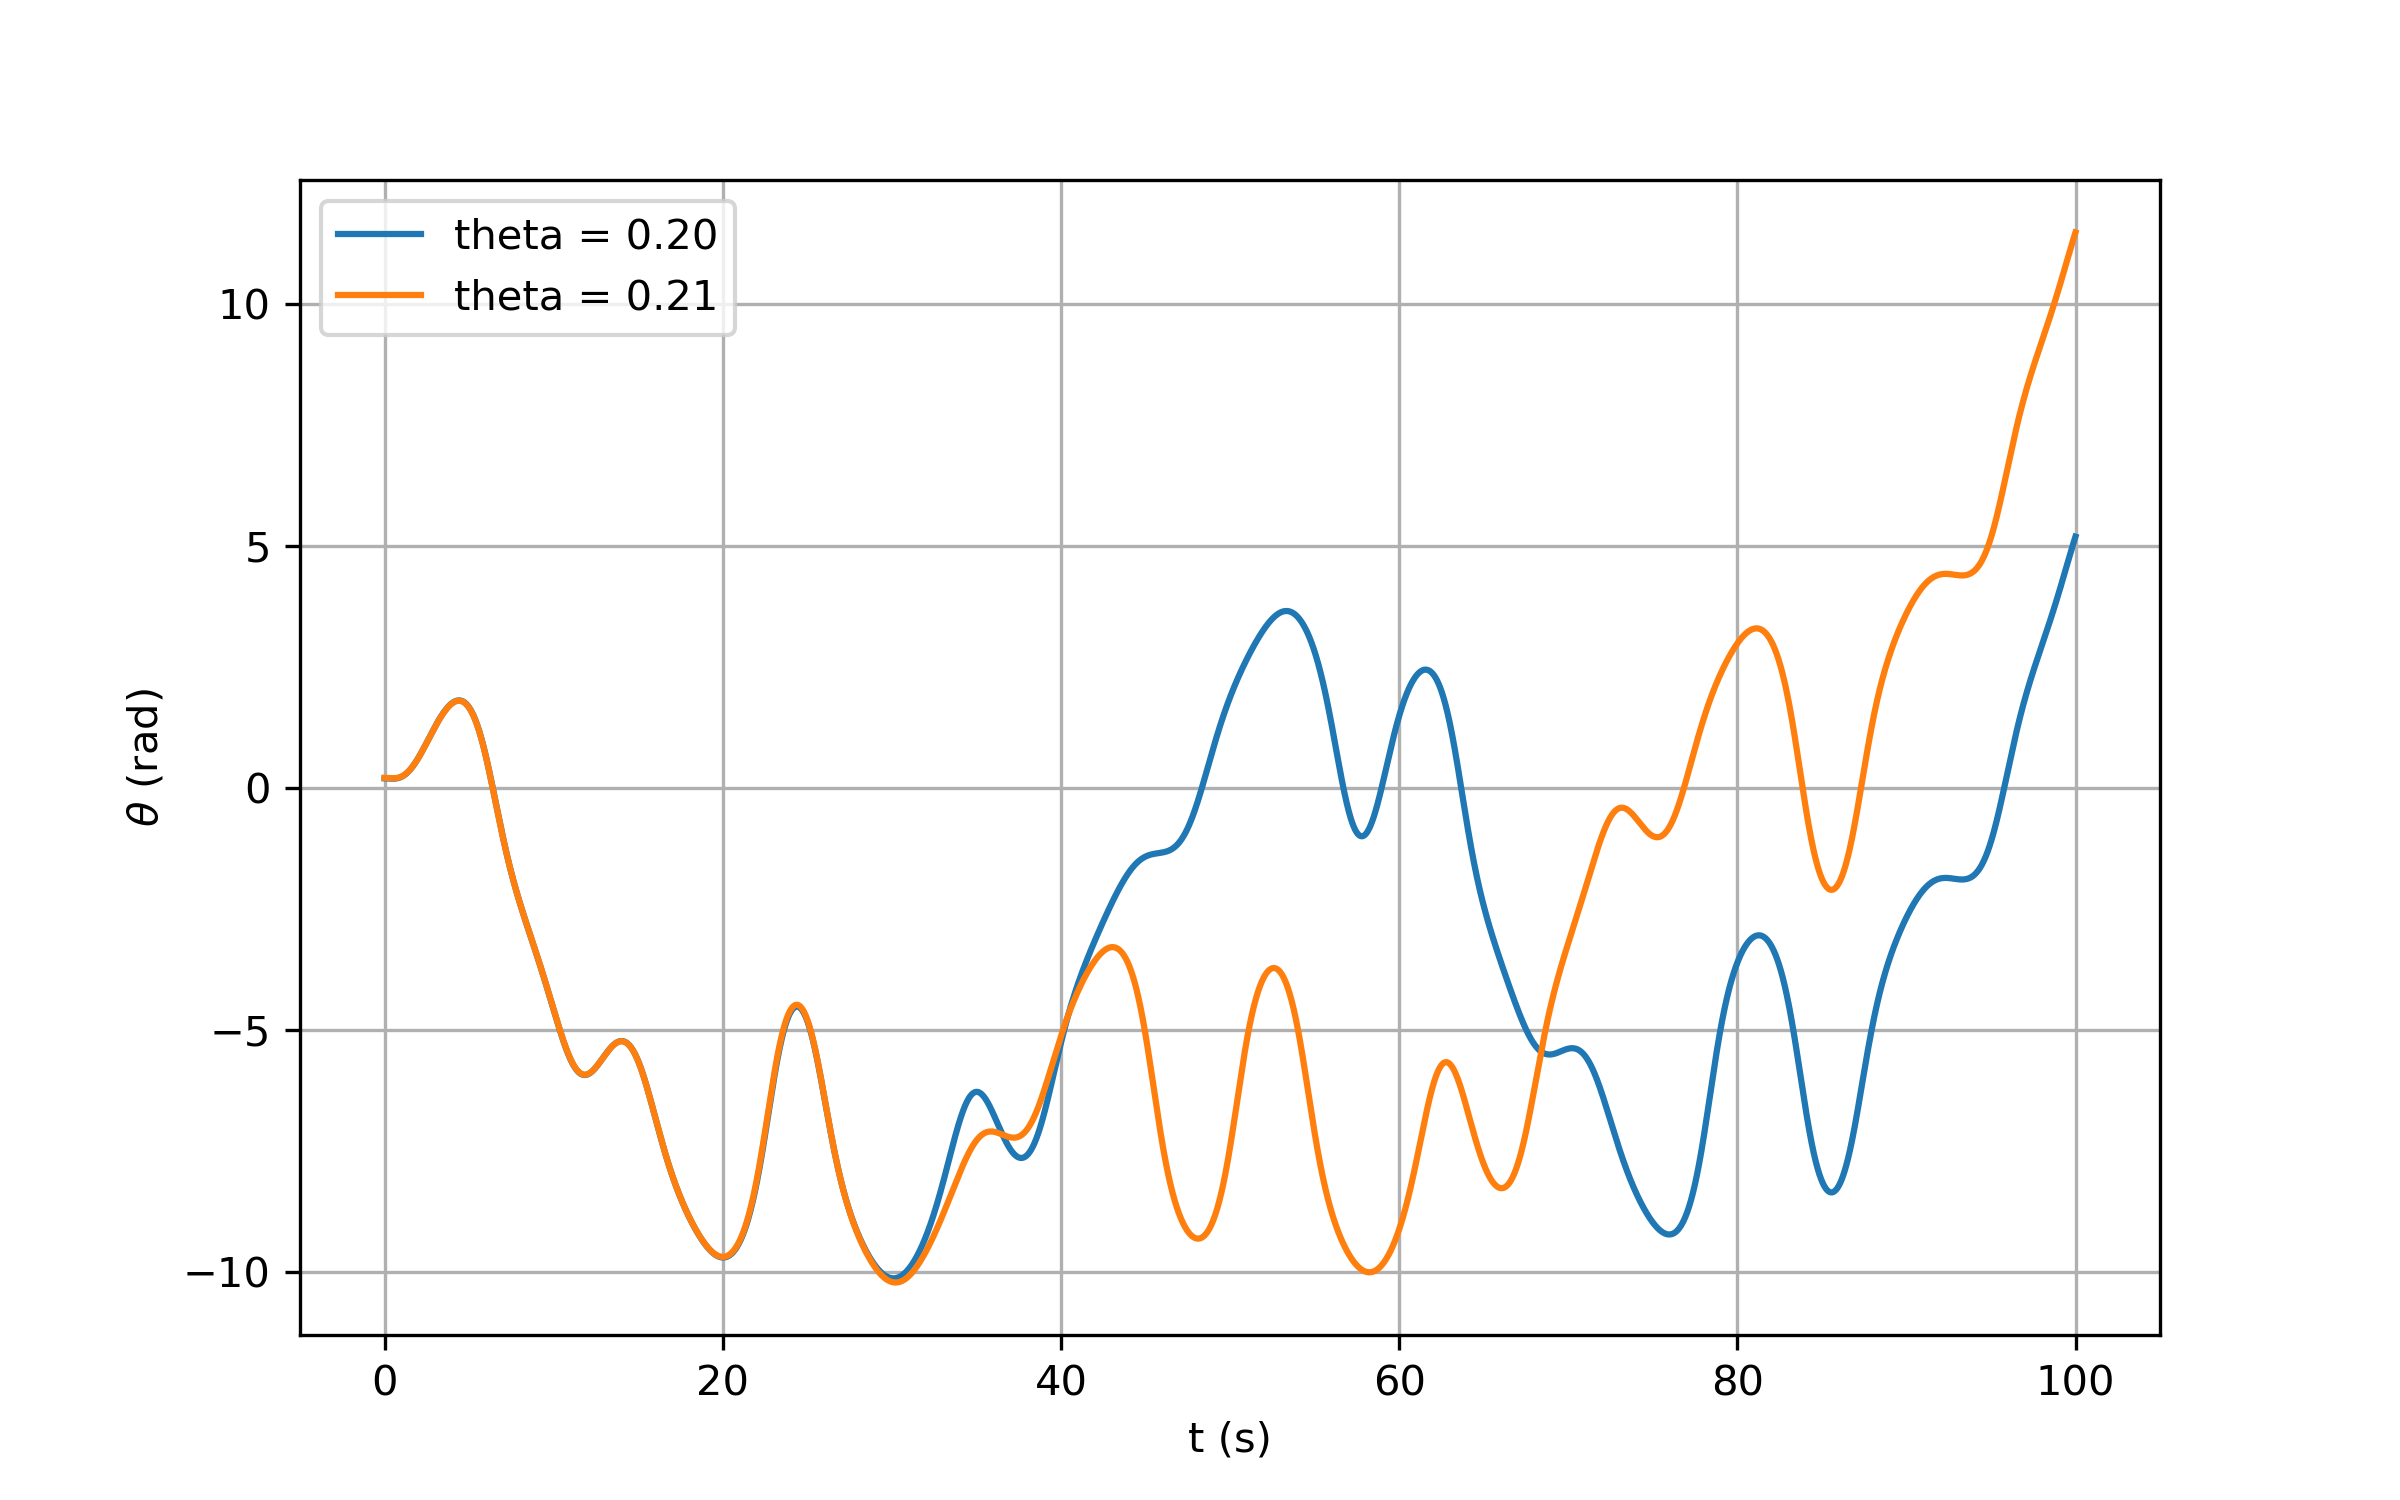
\includegraphics[width=\linewidth]{imagenes_4/comp_ci_0.20.png}
    \caption{$\theta = 0.20$}
\end{subfigure}
\hfill
\begin{subfigure}{0.32\textwidth}
    \centering
    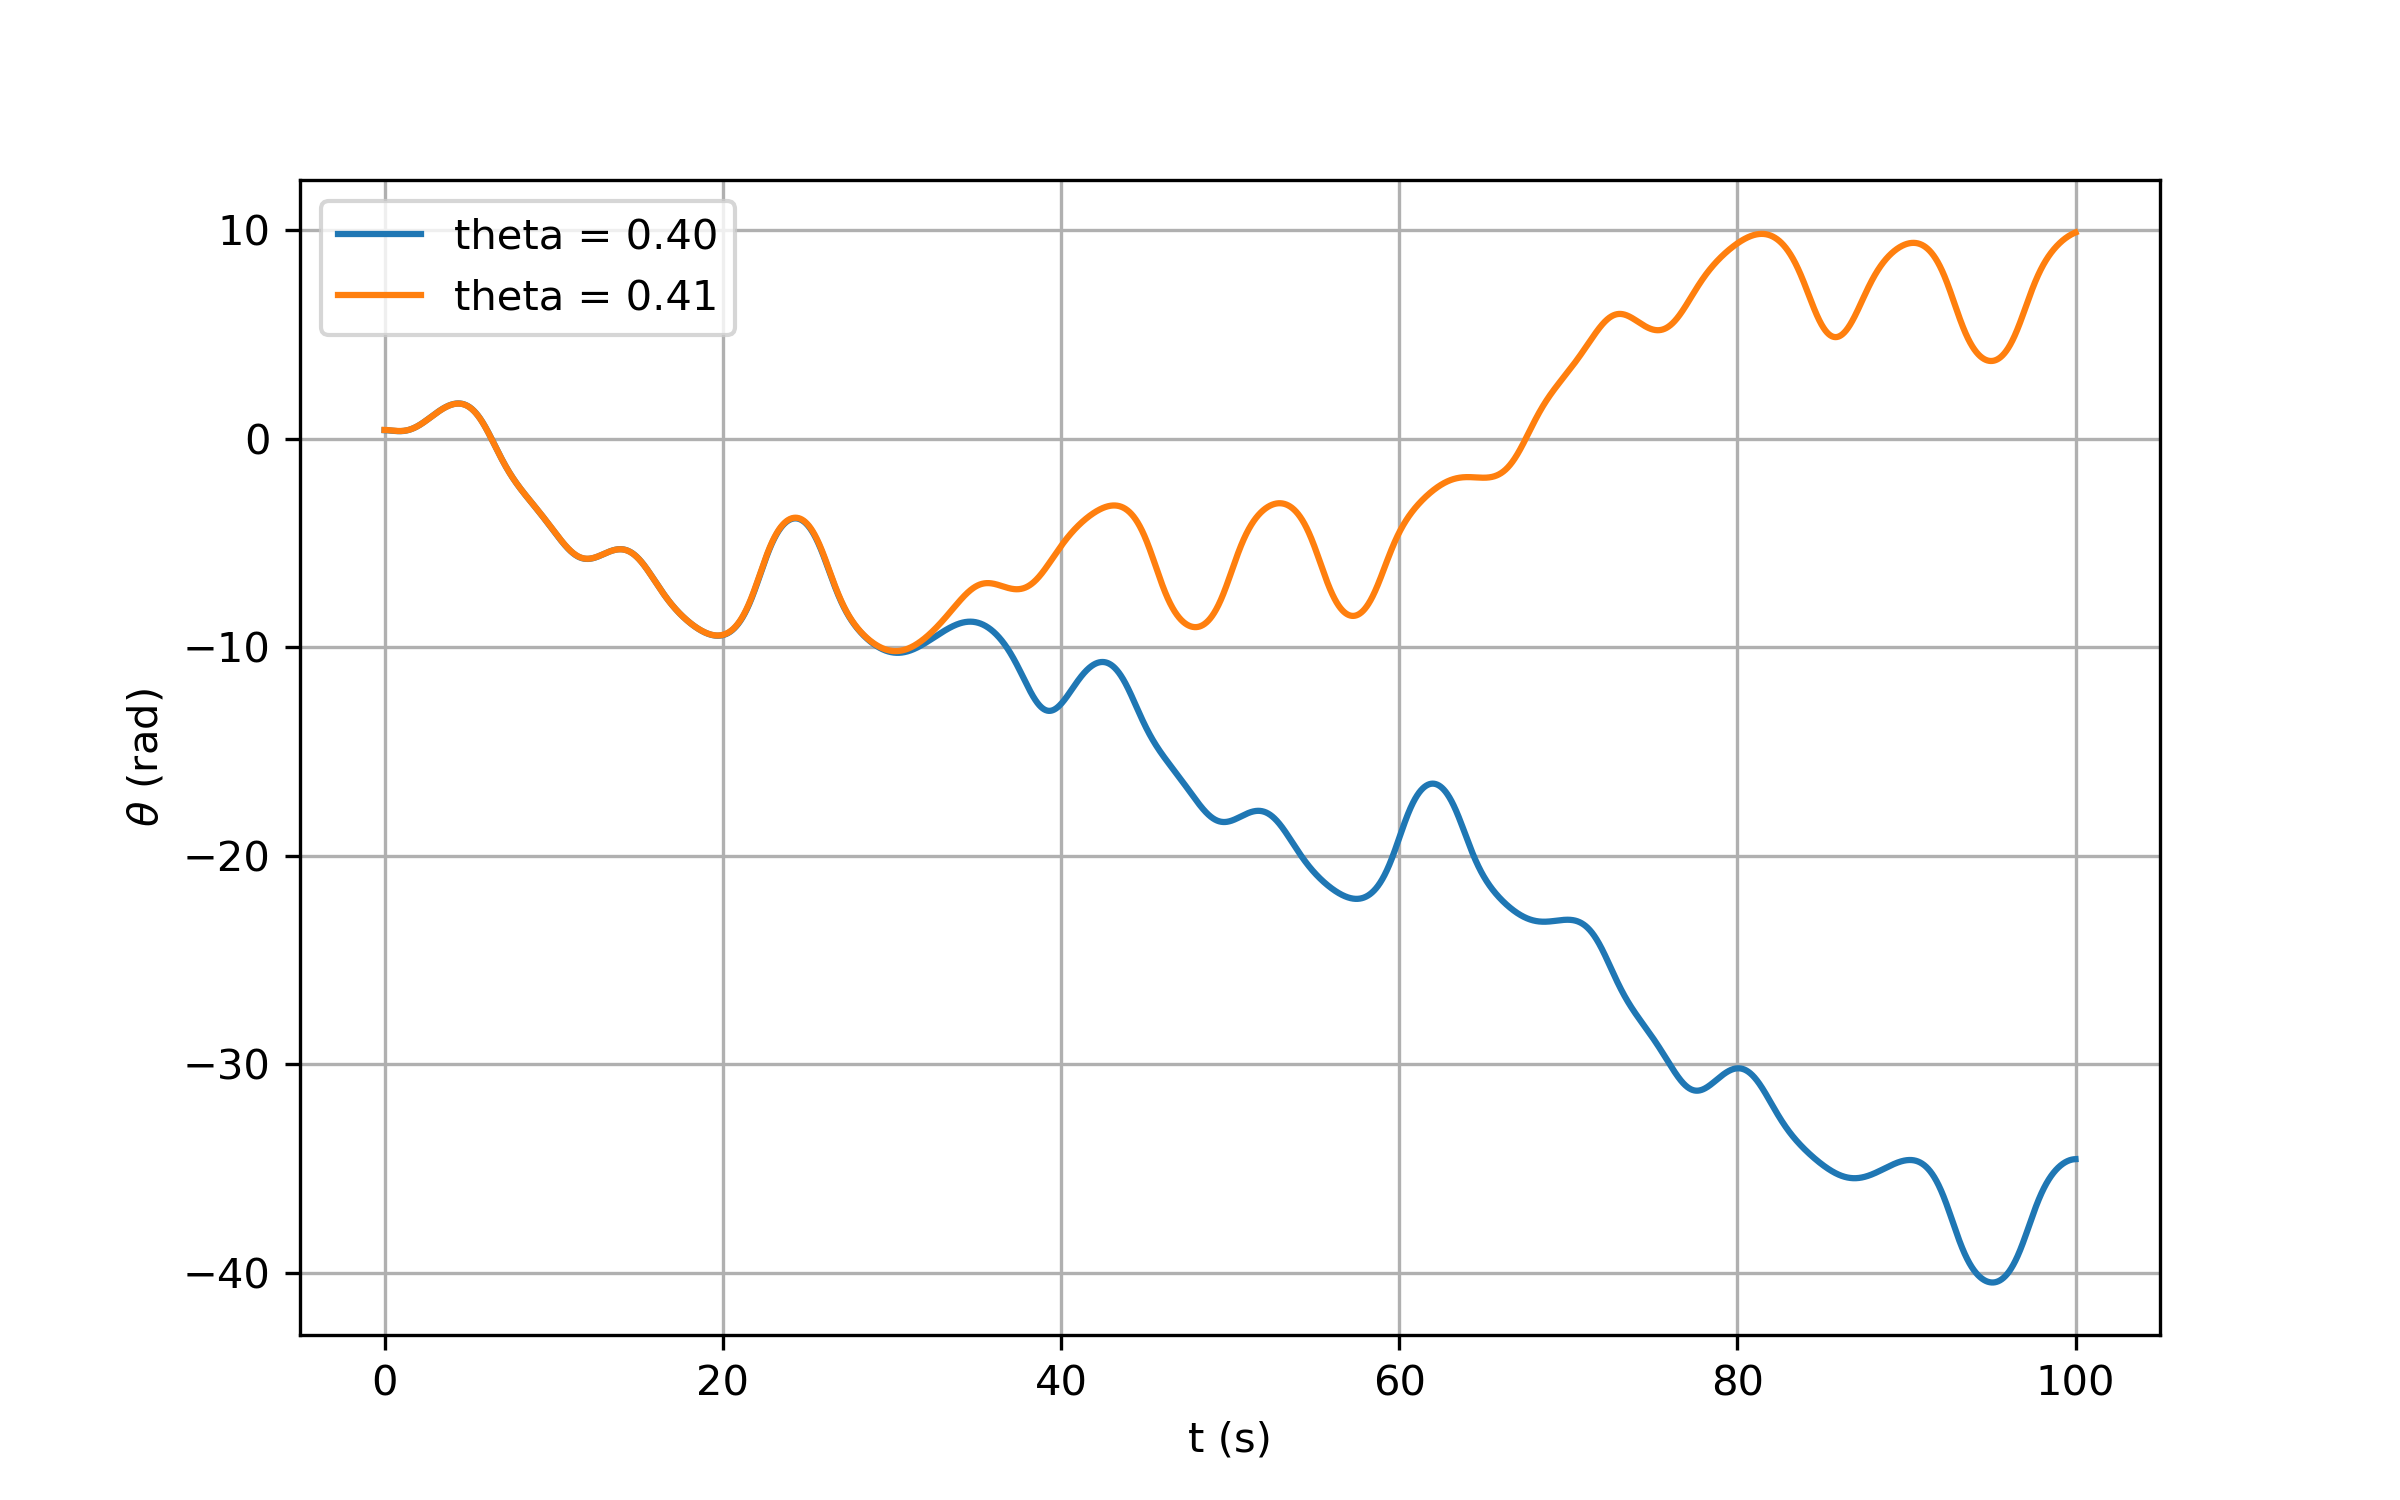
\includegraphics[width=\linewidth]{imagenes_4/comp_ci_0.40.png}
    \caption{$\theta = 0.40$}
\end{subfigure}
\hfill
\begin{subfigure}{0.32\textwidth}
    \centering
    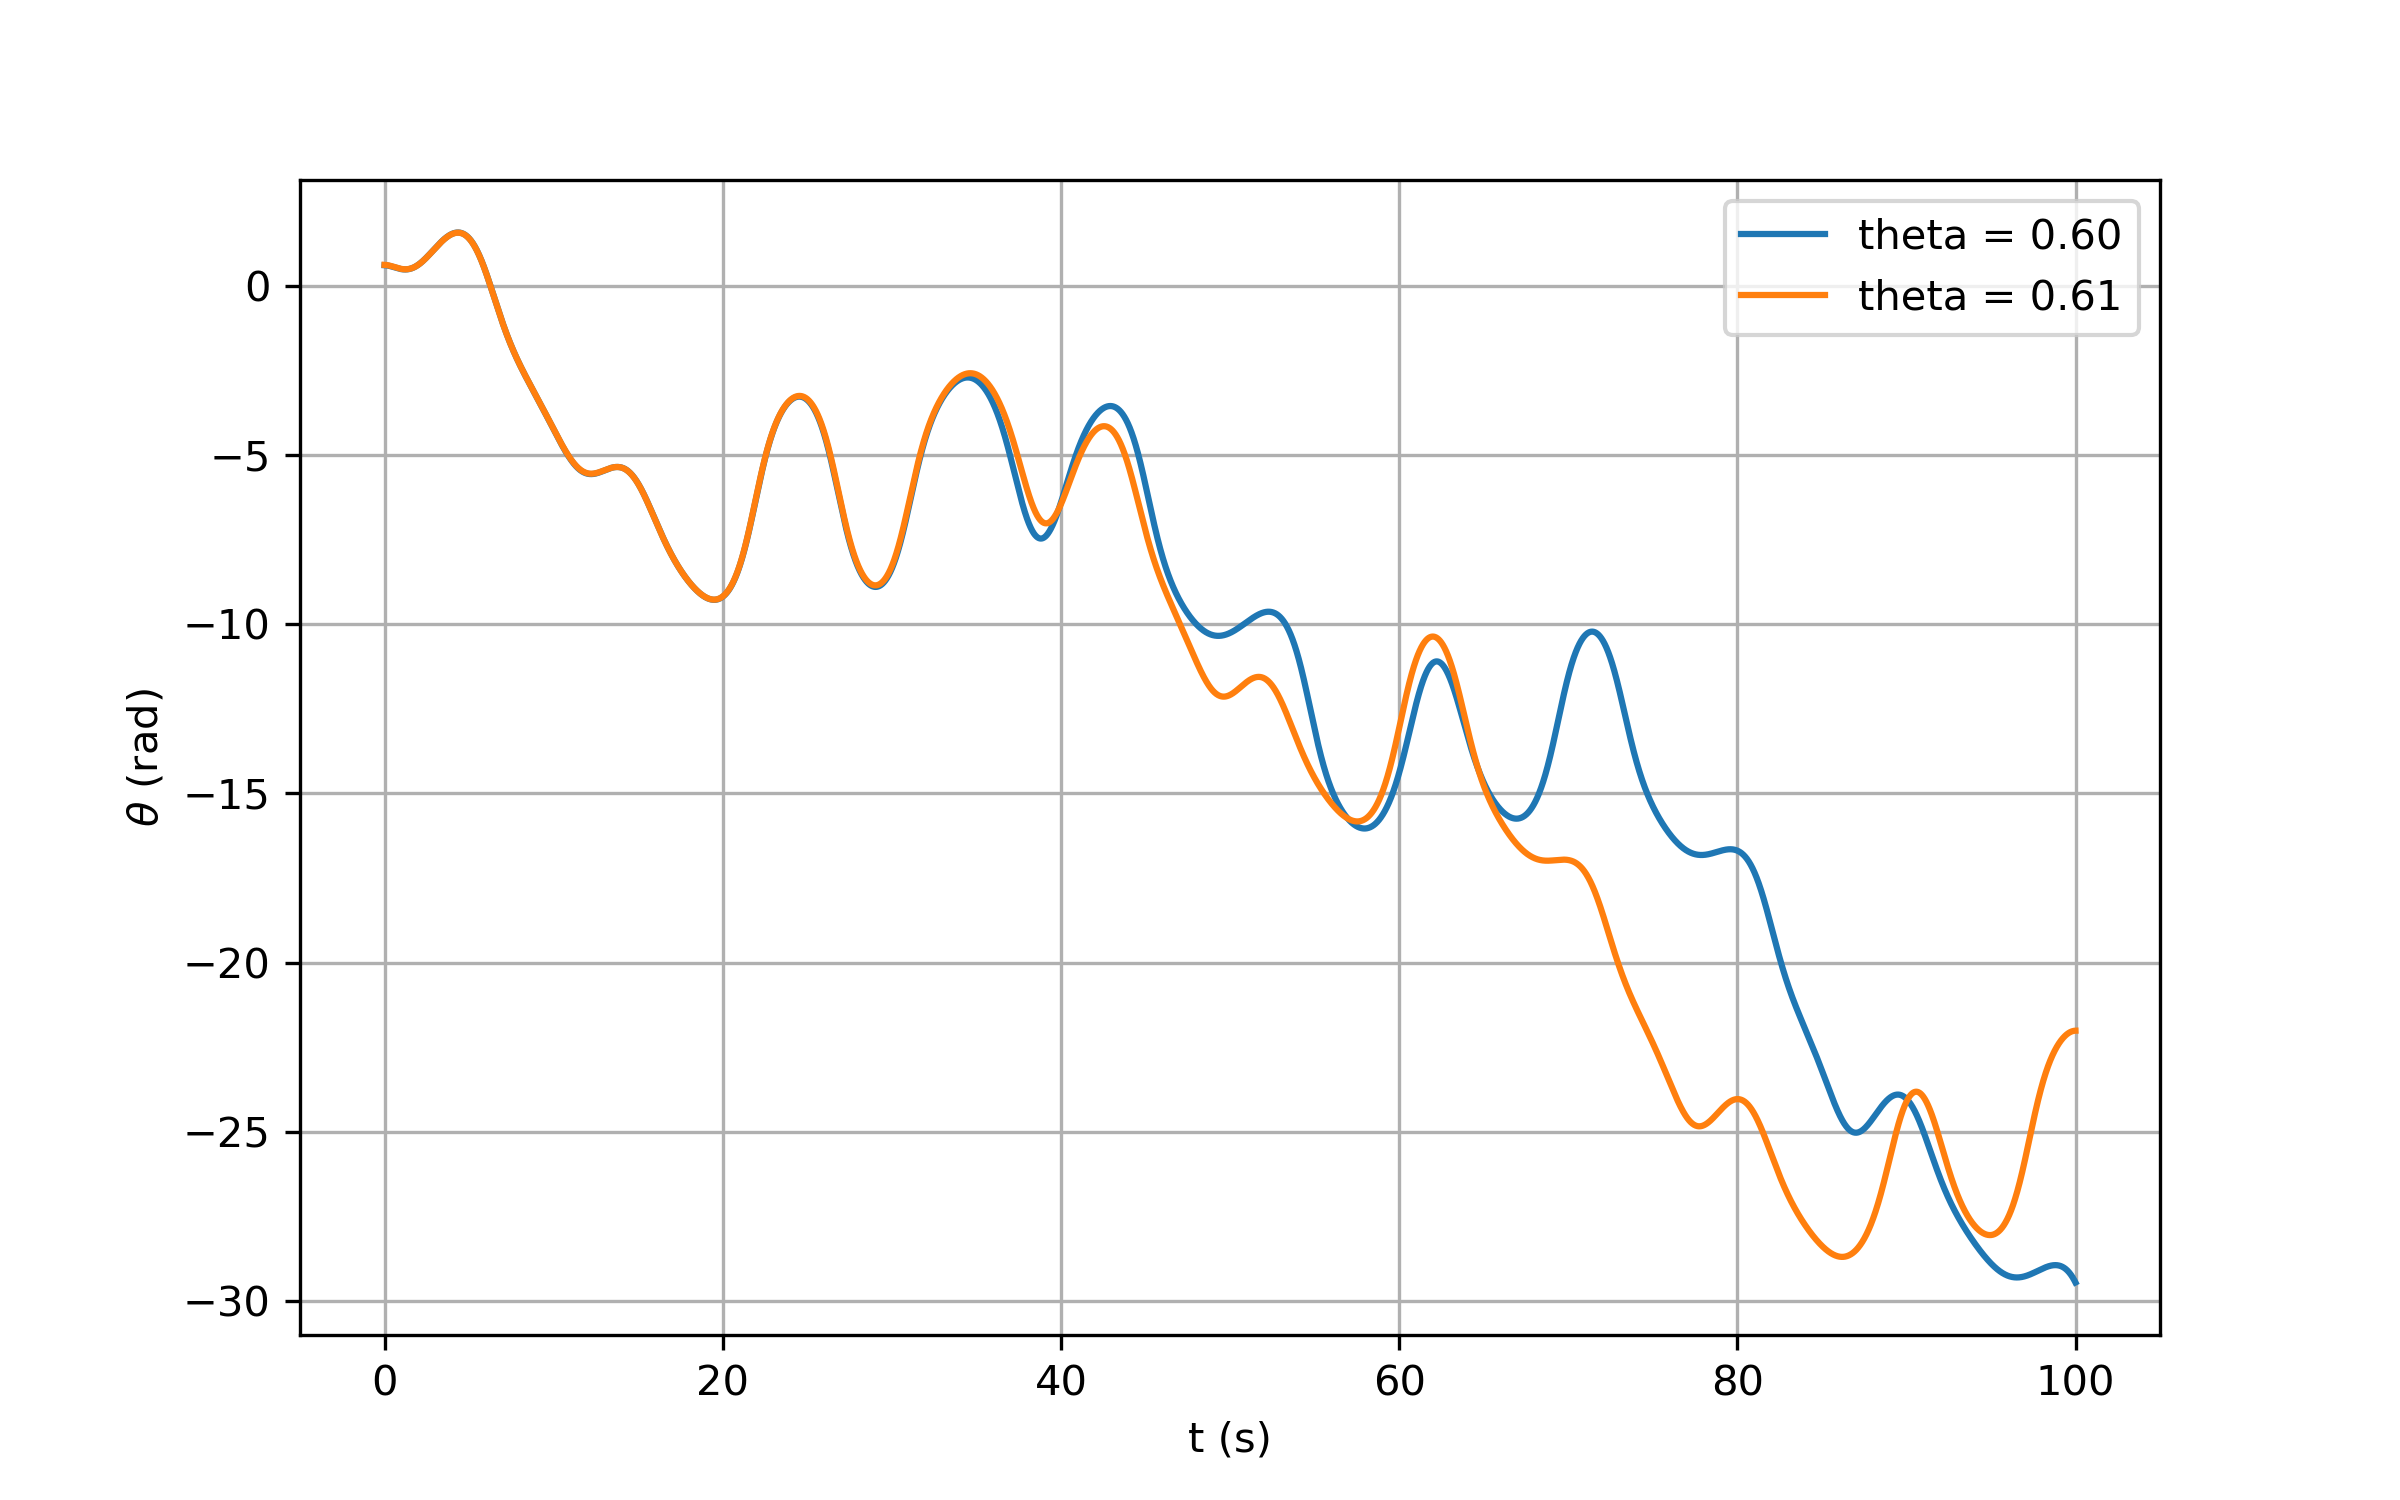
\includegraphics[width=\linewidth]{imagenes_4/comp_ci_0.60.png}
    \caption{$\theta = 0.60$}
\end{subfigure}

\caption{Amplitud angular del péndulo en función del tiempo}
\label{fig:comparacion}
\end{figure}

\begin{figure}[H]
\centering
\begin{subfigure}{0.32\textwidth}
    \centering
    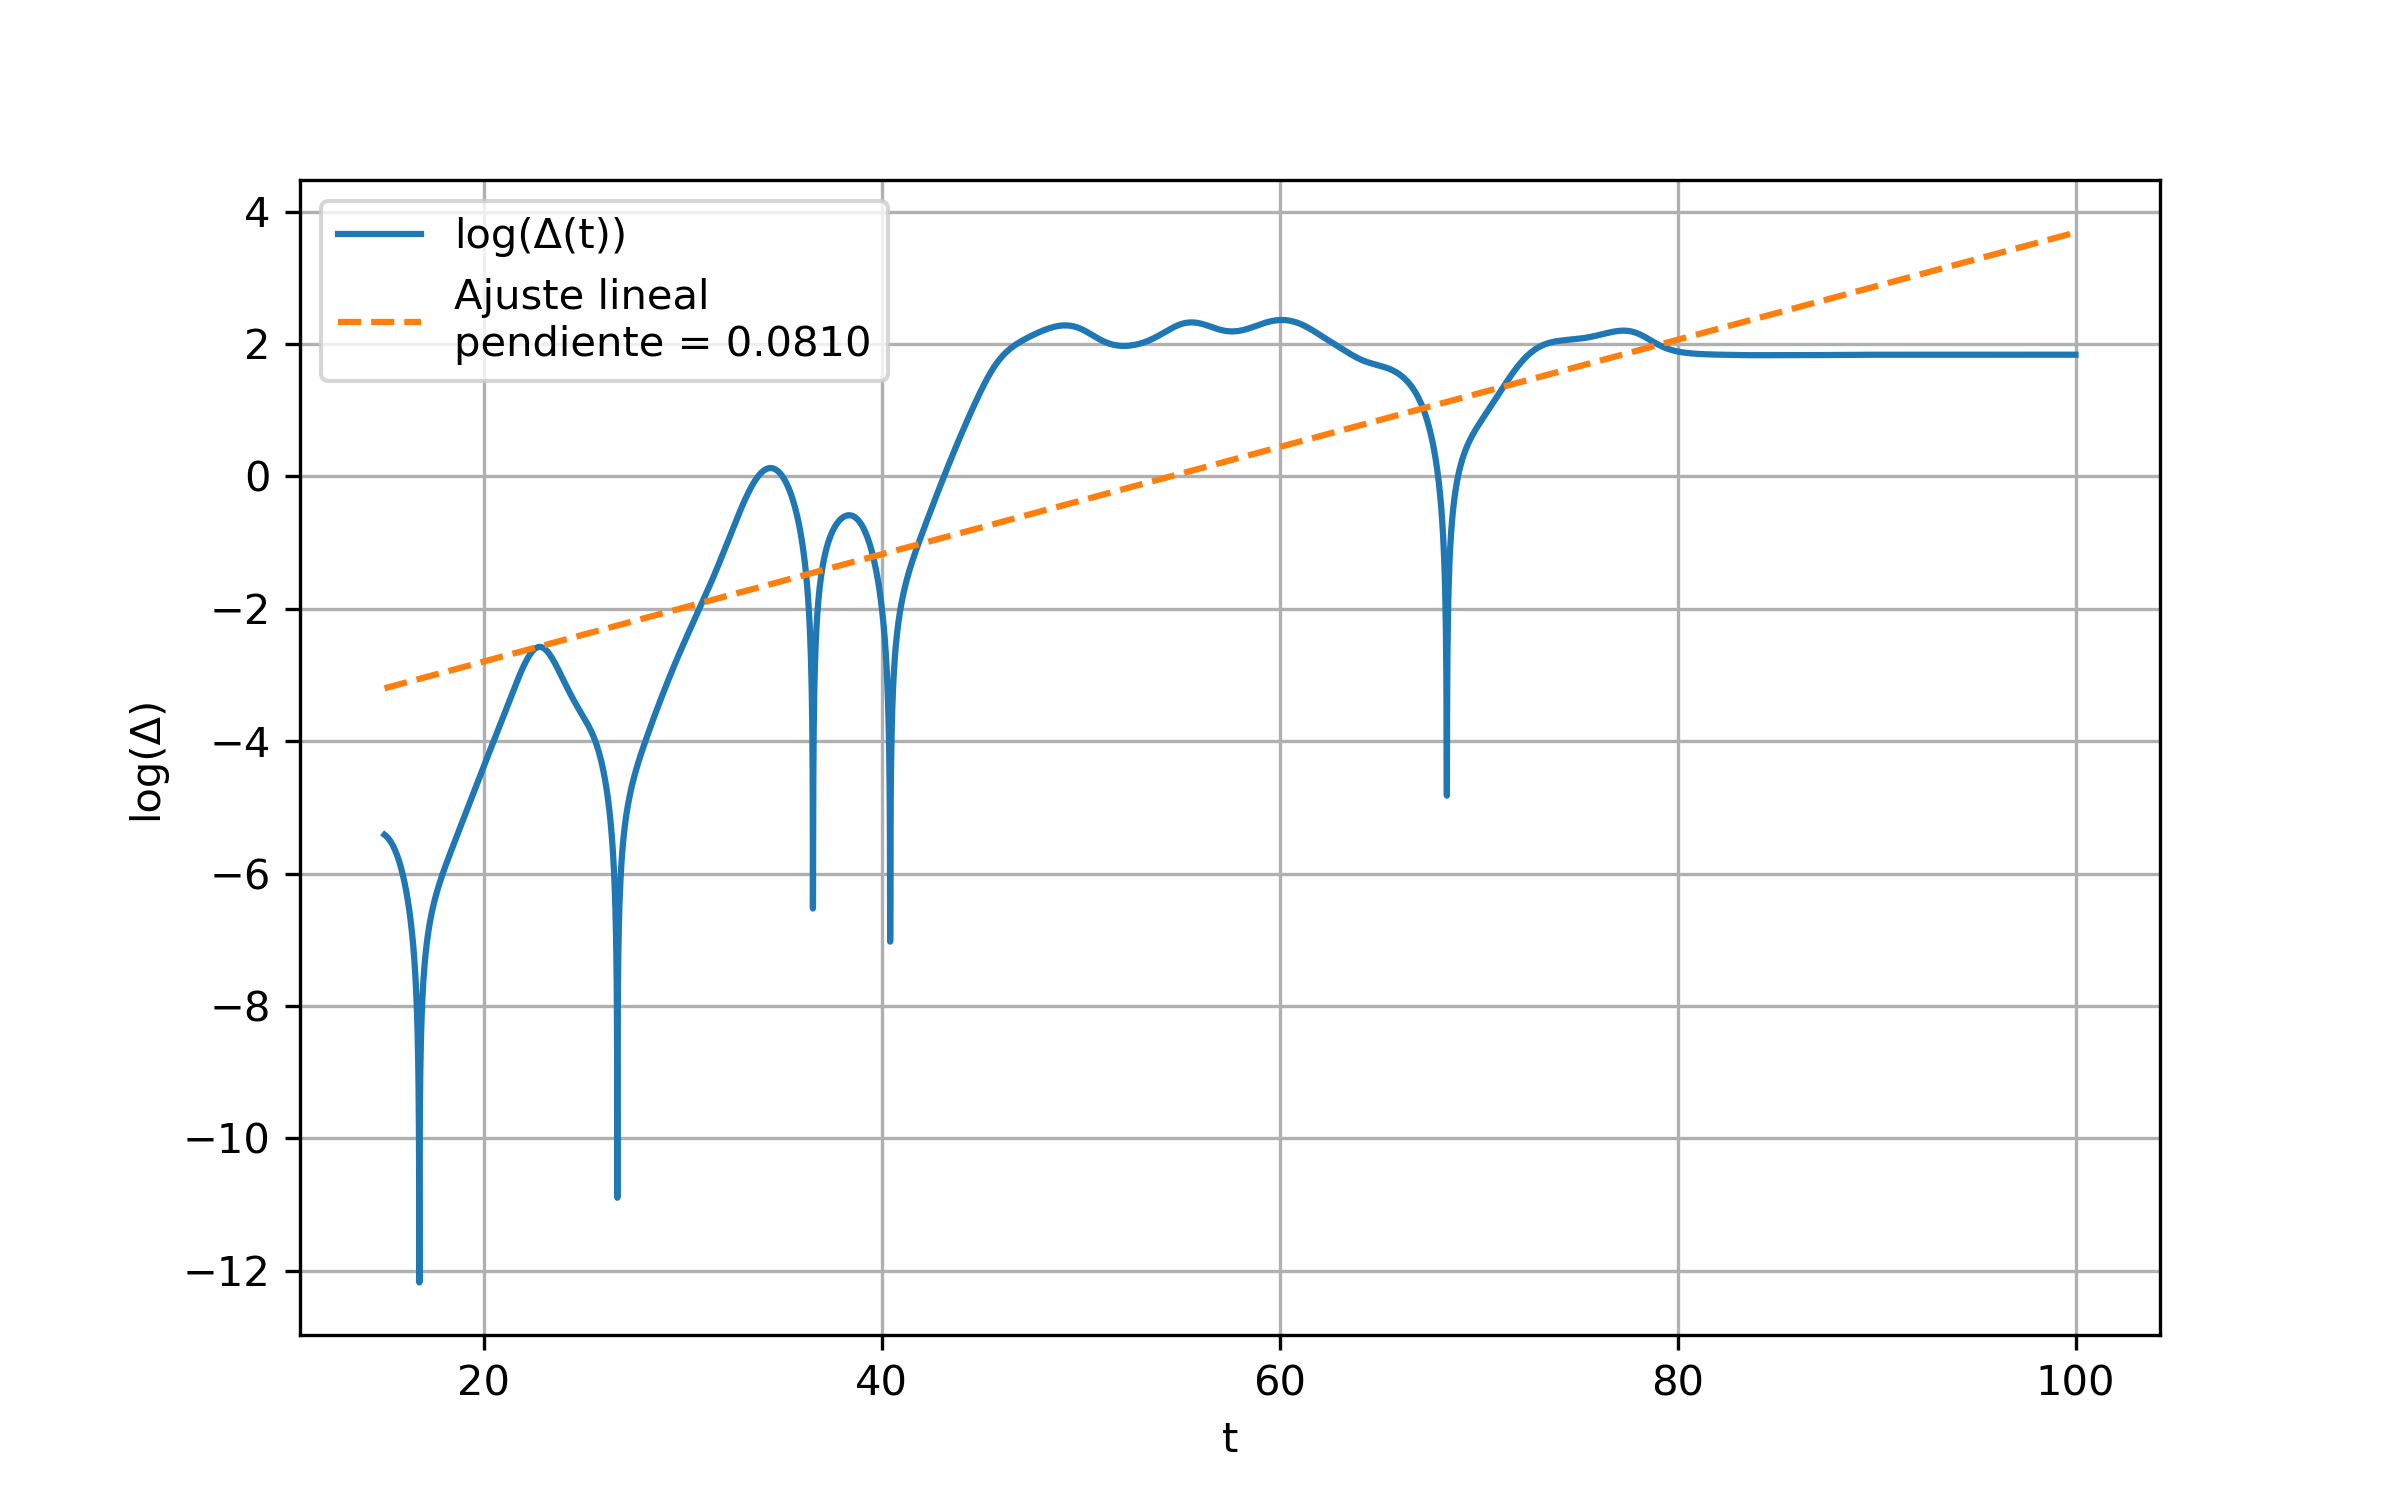
\includegraphics[width=\linewidth]{imagenes_4/apartado_a_theta_0.20.png}
    \caption{$\theta = 0.20$}
\end{subfigure}
\hfill
\begin{subfigure}{0.32\textwidth}
    \centering
    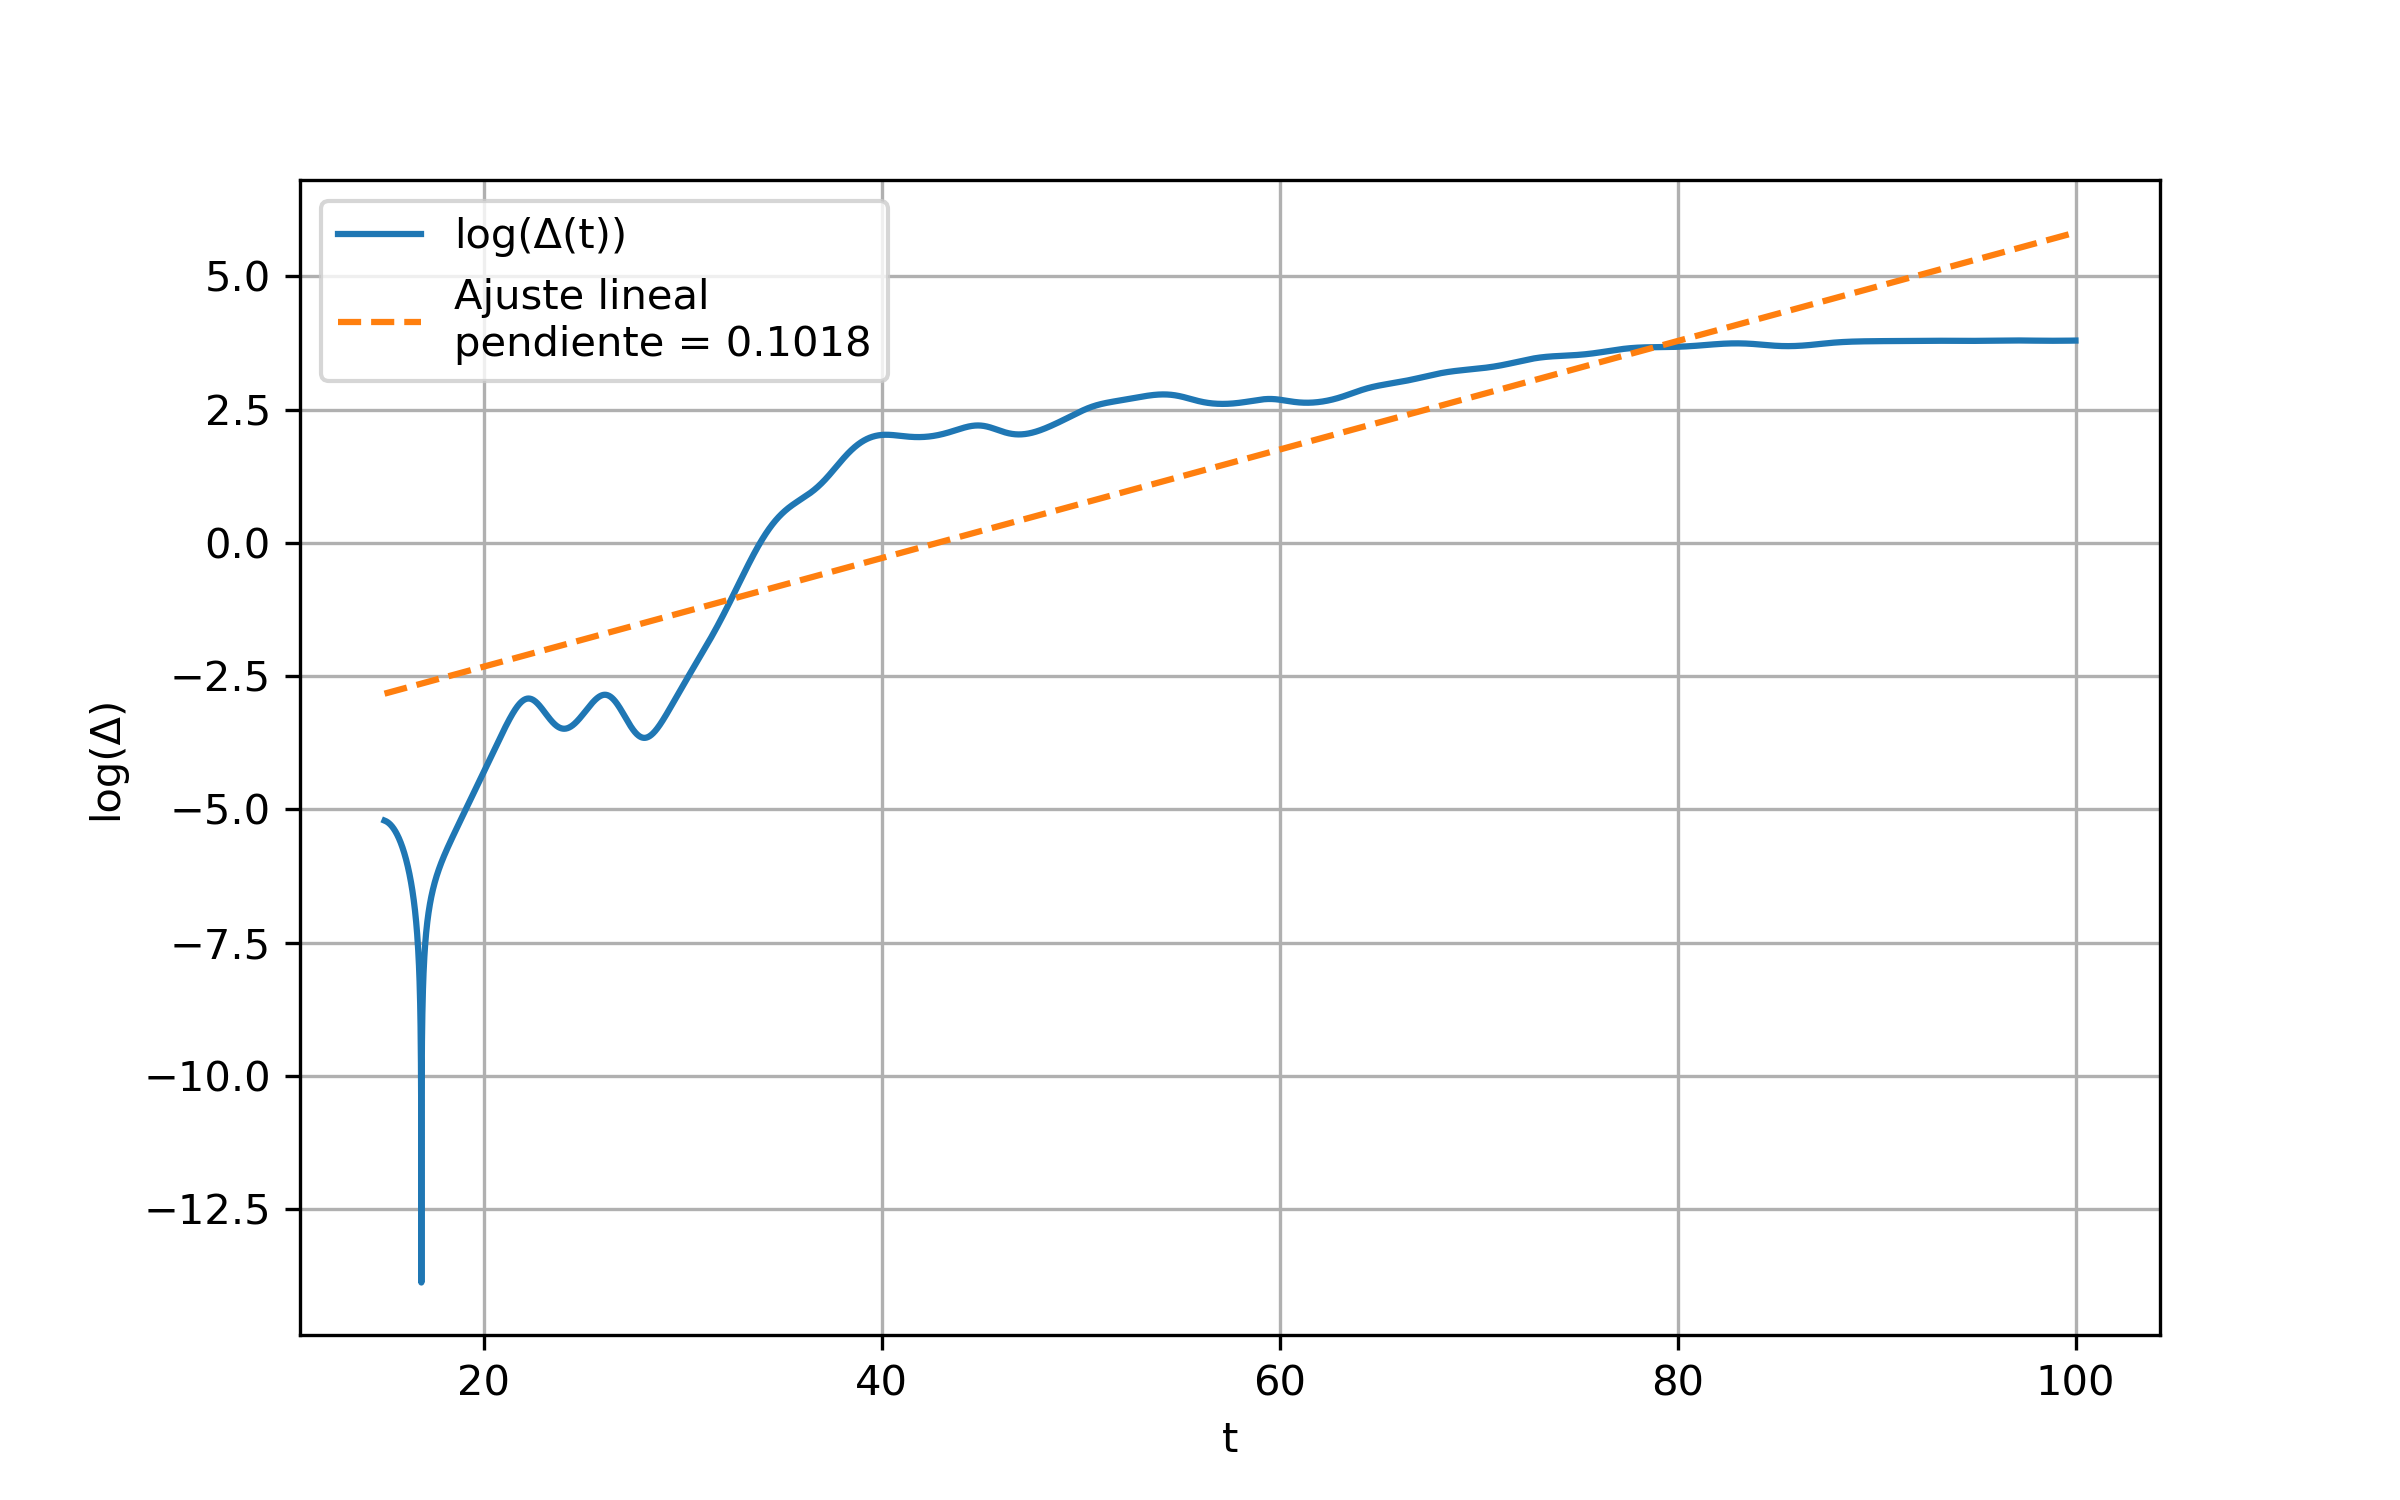
\includegraphics[width=\linewidth]{imagenes_4/apartado_a_theta_0.40.png}
    \caption{$\theta = 0.40$}
\end{subfigure}
\hfill
\begin{subfigure}{0.32\textwidth}
    \centering
    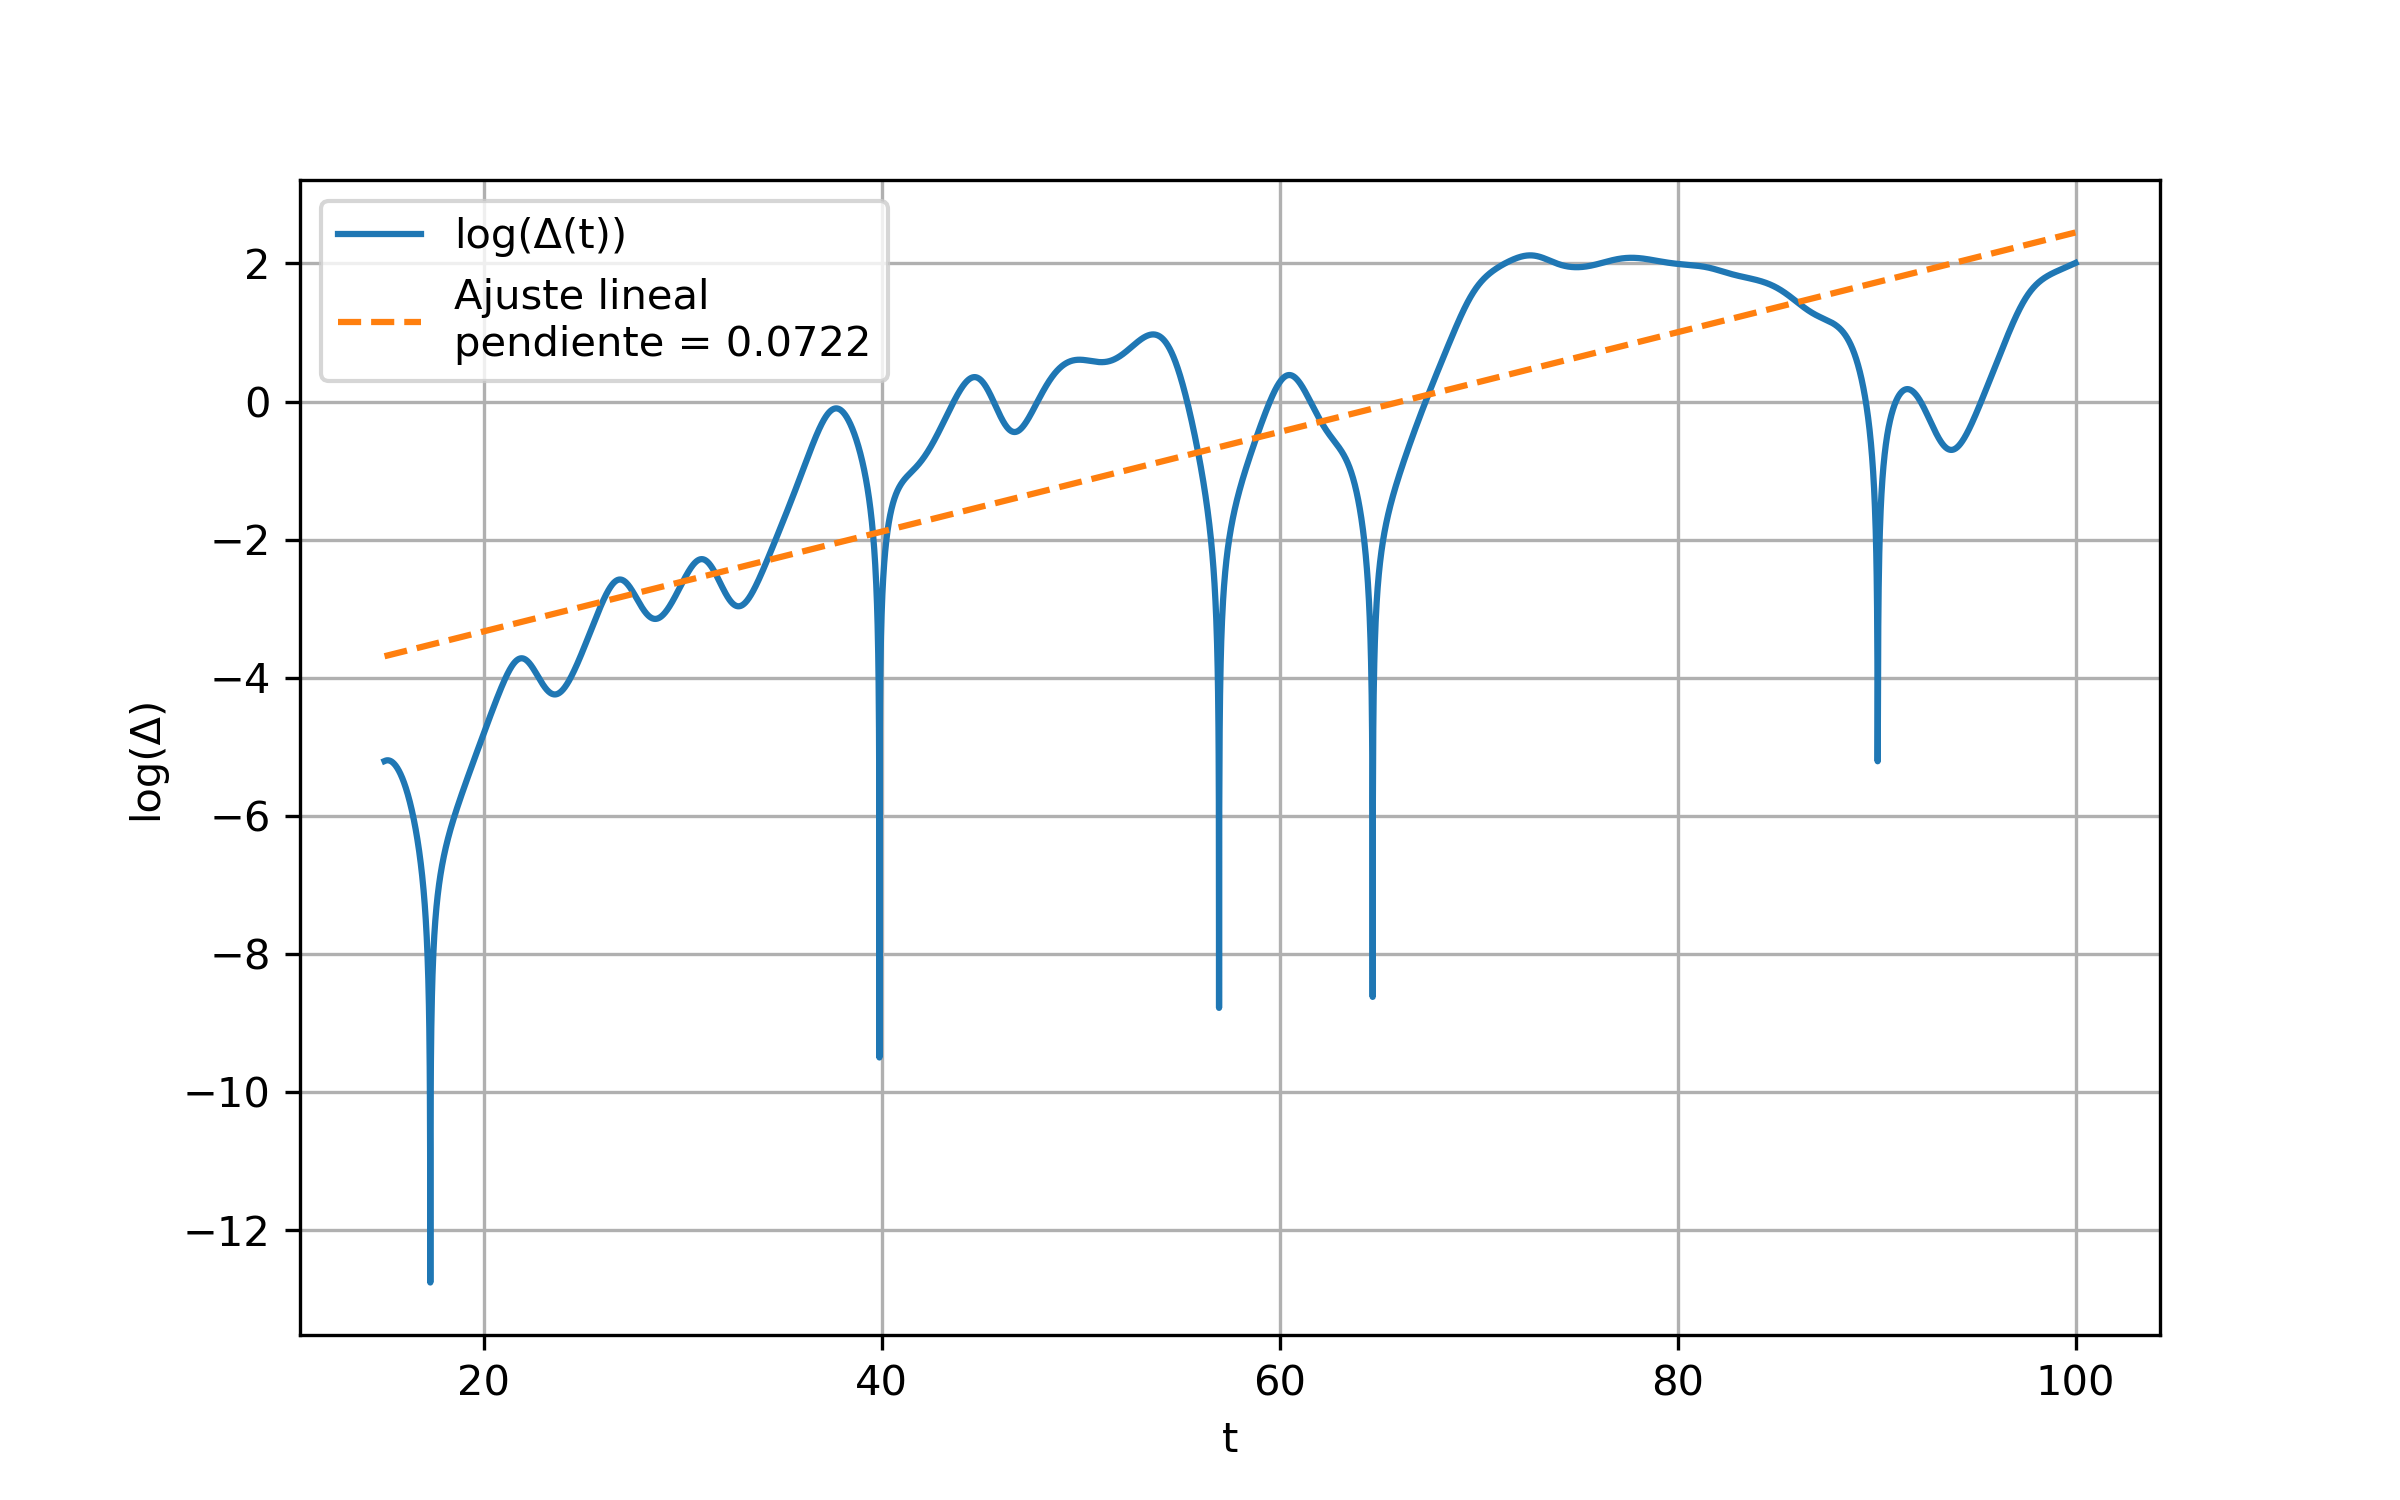
\includegraphics[width=\linewidth]{imagenes_4/apartado_a_theta_0.60.png}
    \caption{$\theta = 0.60$}
\end{subfigure}

\caption{Obtención de los exponentes de Lyapunov}
\label{fig:comparacion}
\end{figure}

El valor estimado del exponente de Lyapunov obtenido es:

\[
\lambda = 0.085 \pm 0.012>0
\]

lo que indica divergencia exponencial entre trayectorias y por tanto comportamiento caótico.

\subsection{Sensibilidad al amortiguamiento}

En el segundo experimento se analizaron dos péndulos que parten de posiciones casi idénticas (como en el apartado anterior) y además con coeficientes de amortiguamiento ligeramente diferentes (separados $\Delta q$). El coeficiente 

\begin{figure}[H]
\centering
\begin{subfigure}{0.32\textwidth}
    \centering
    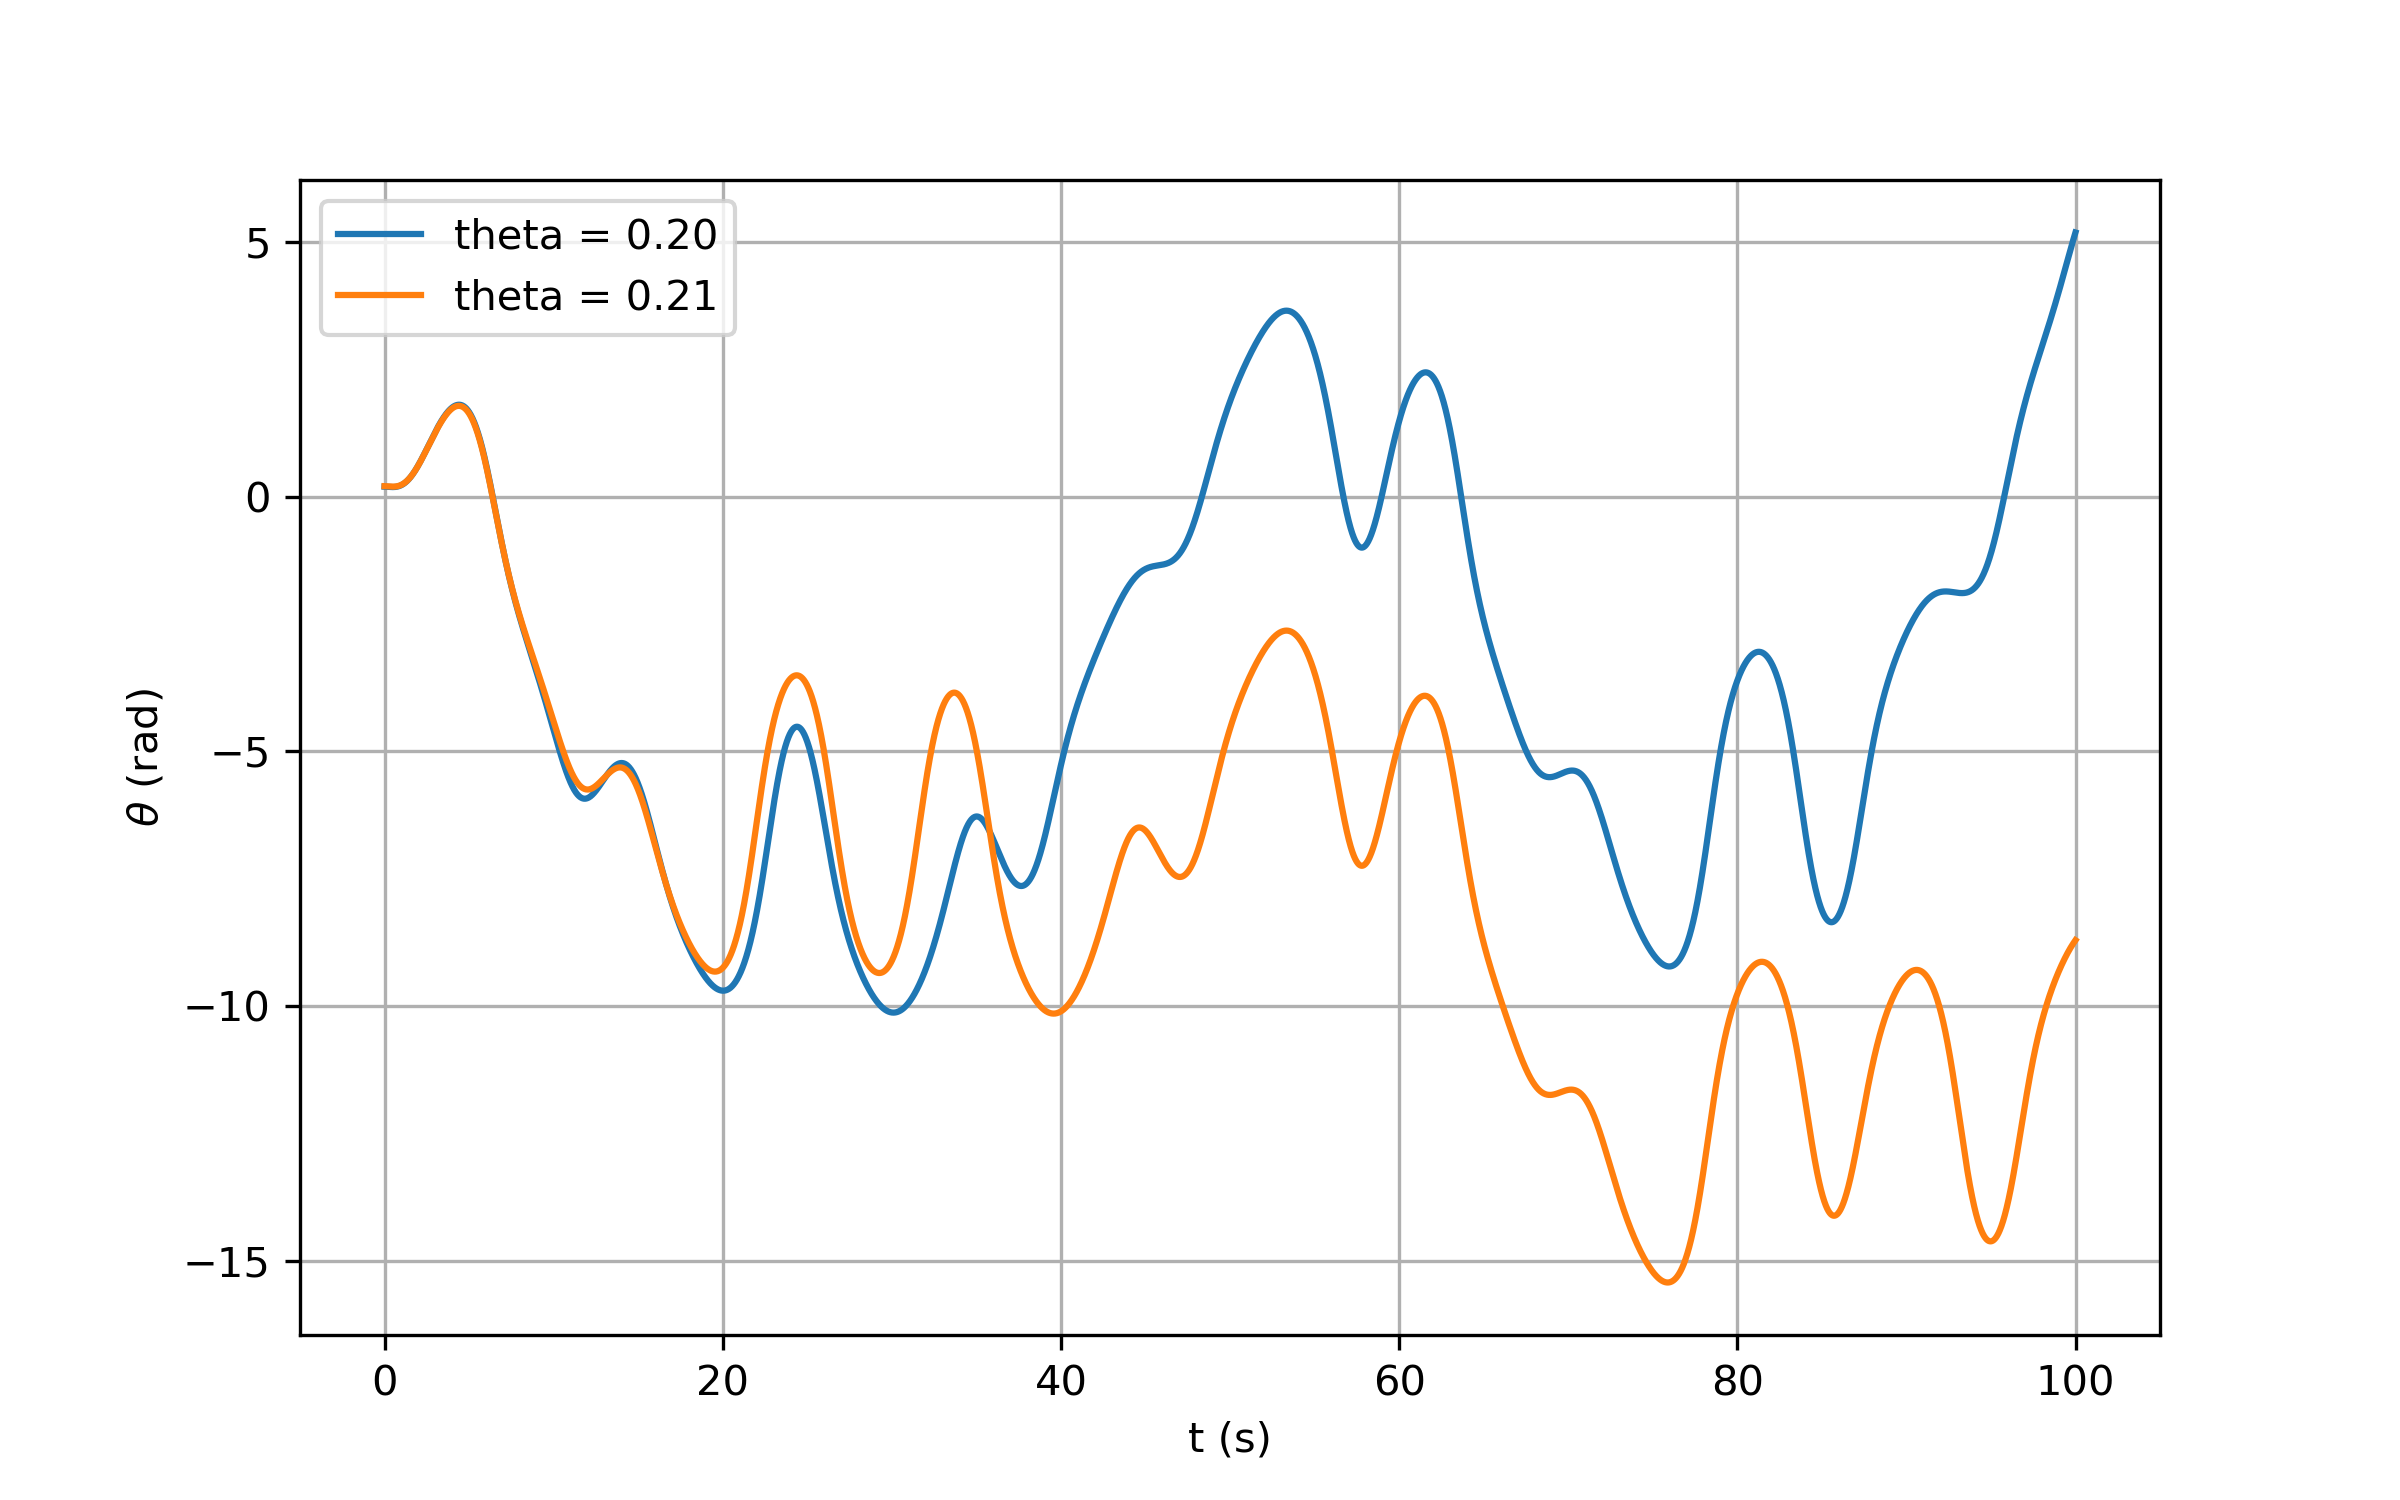
\includegraphics[width=\linewidth]{imagenes_4/comp_ci_b_0.20.png}
    \caption{$\theta = 0.20$}
\end{subfigure}
\hfill
\begin{subfigure}{0.32\textwidth}
    \centering
    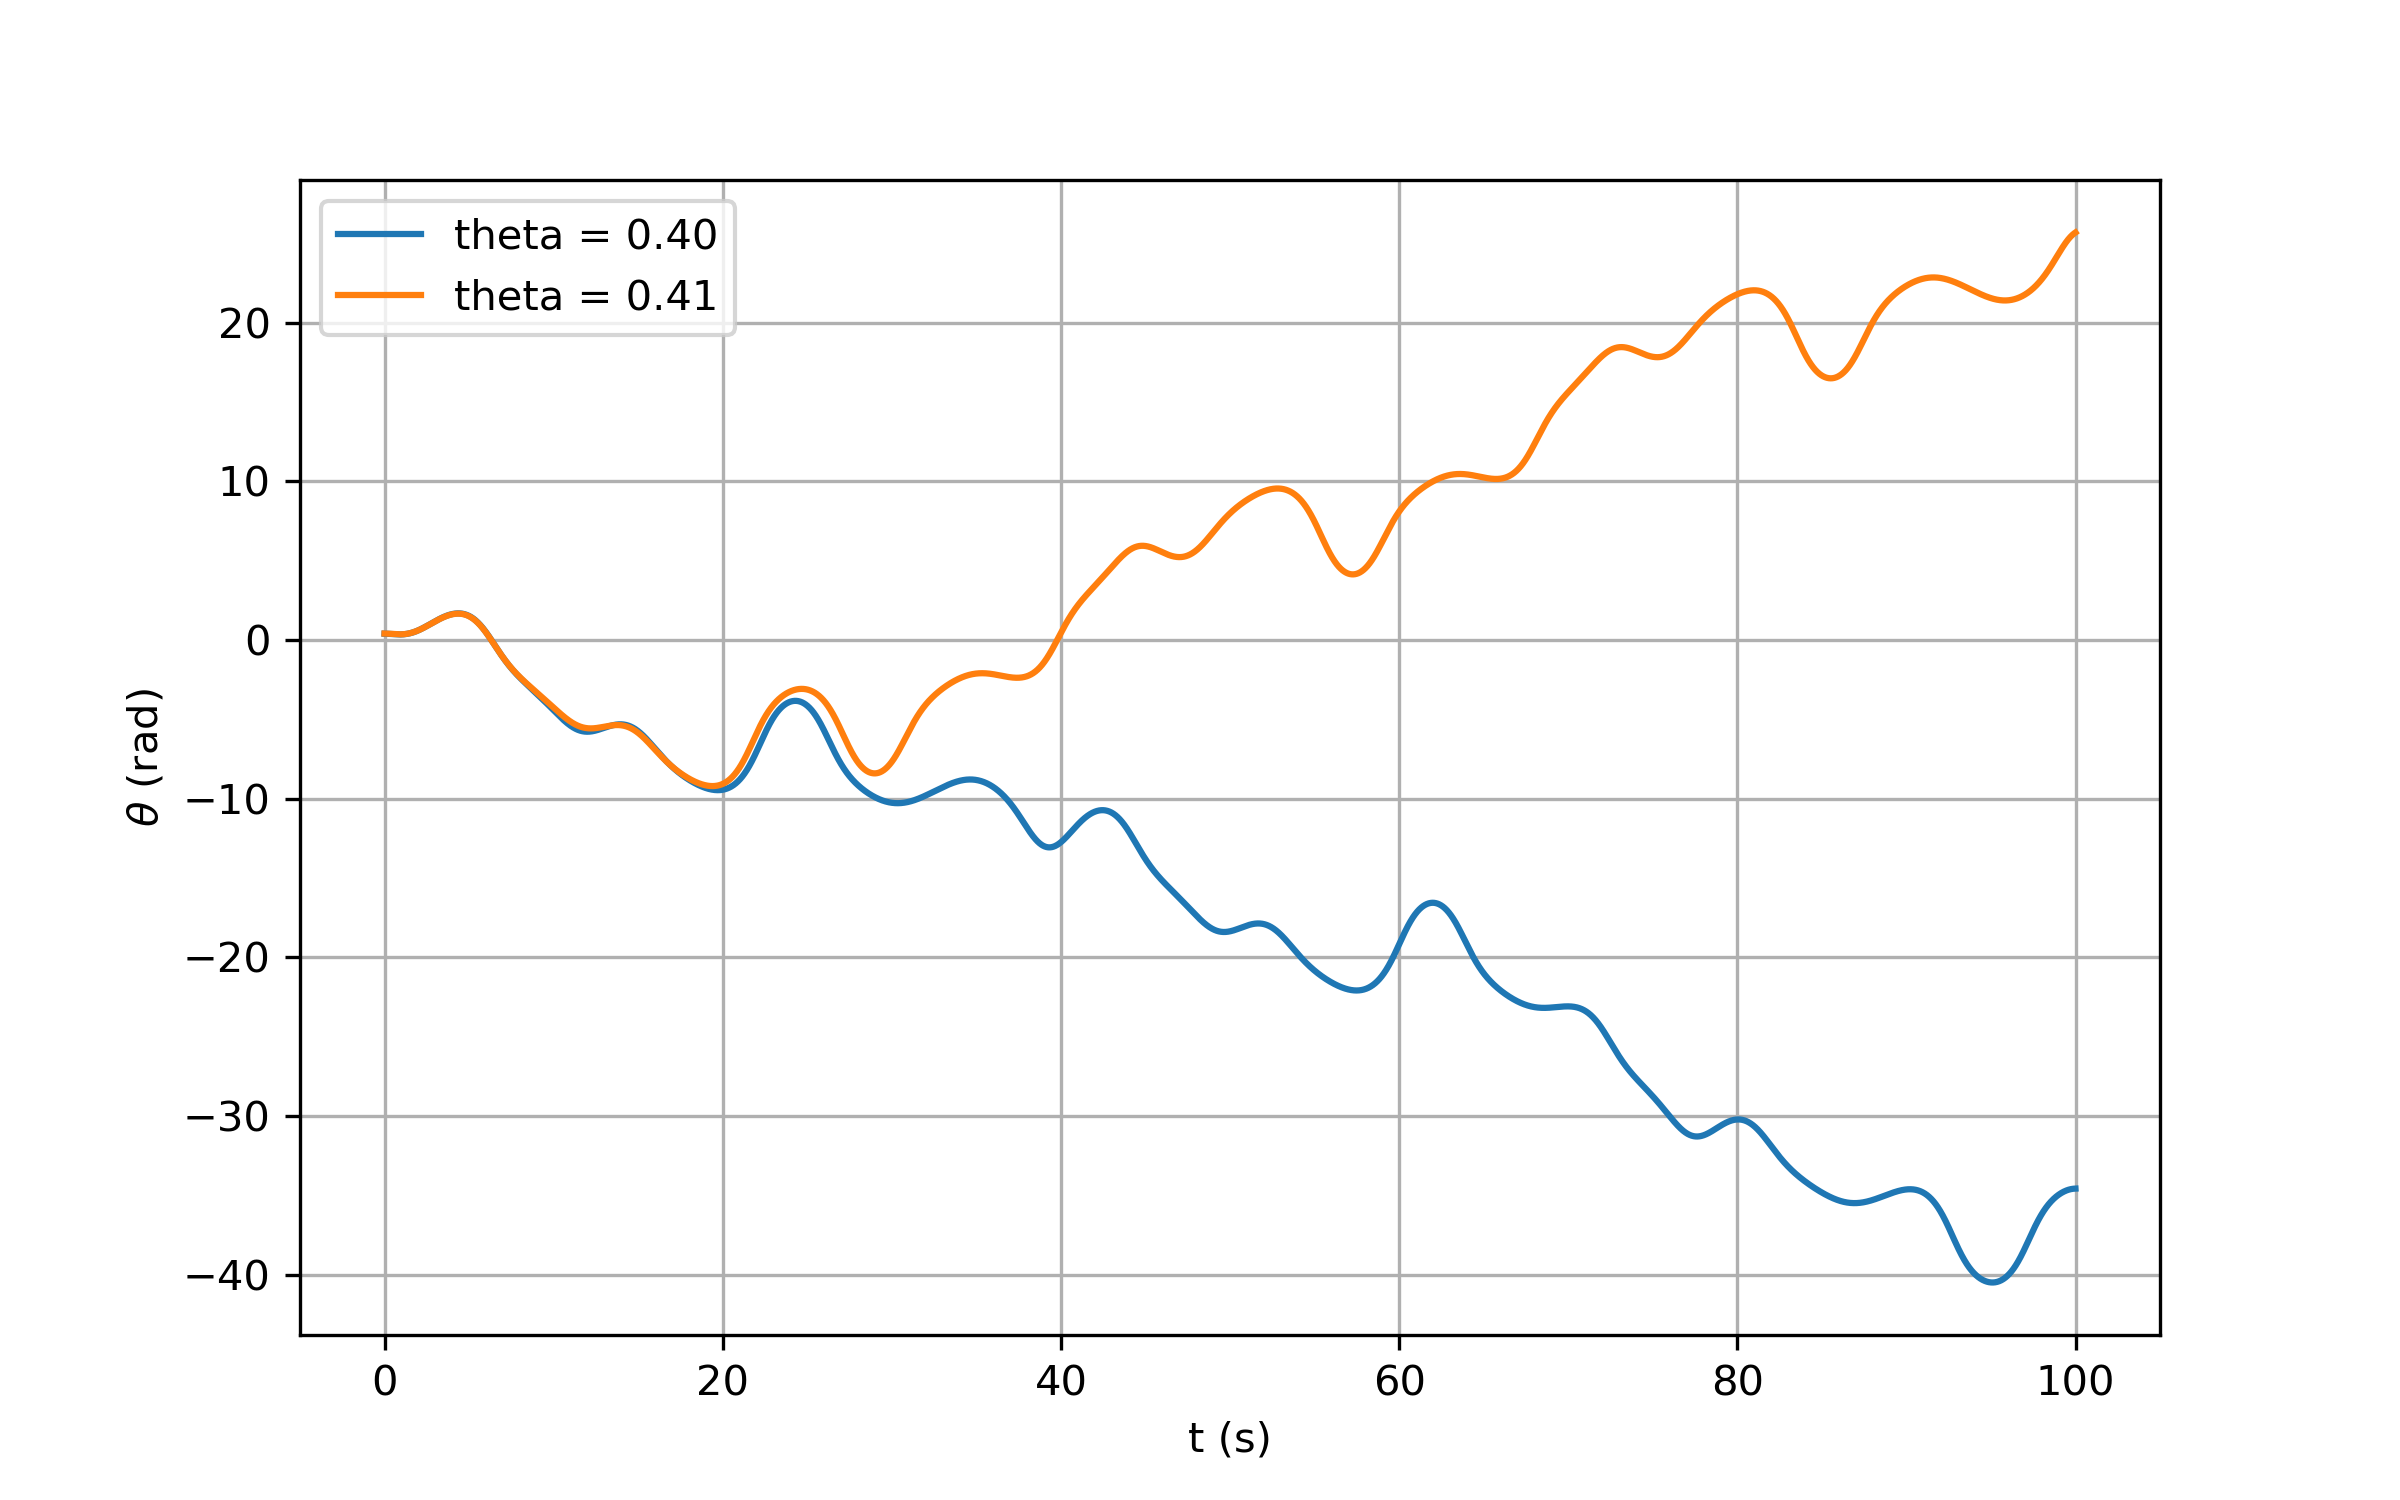
\includegraphics[width=\linewidth]{imagenes_4/comp_ci_b_0.40.png}
    \caption{$\theta = 0.40$}
\end{subfigure}
\hfill
\begin{subfigure}{0.32\textwidth}
    \centering
    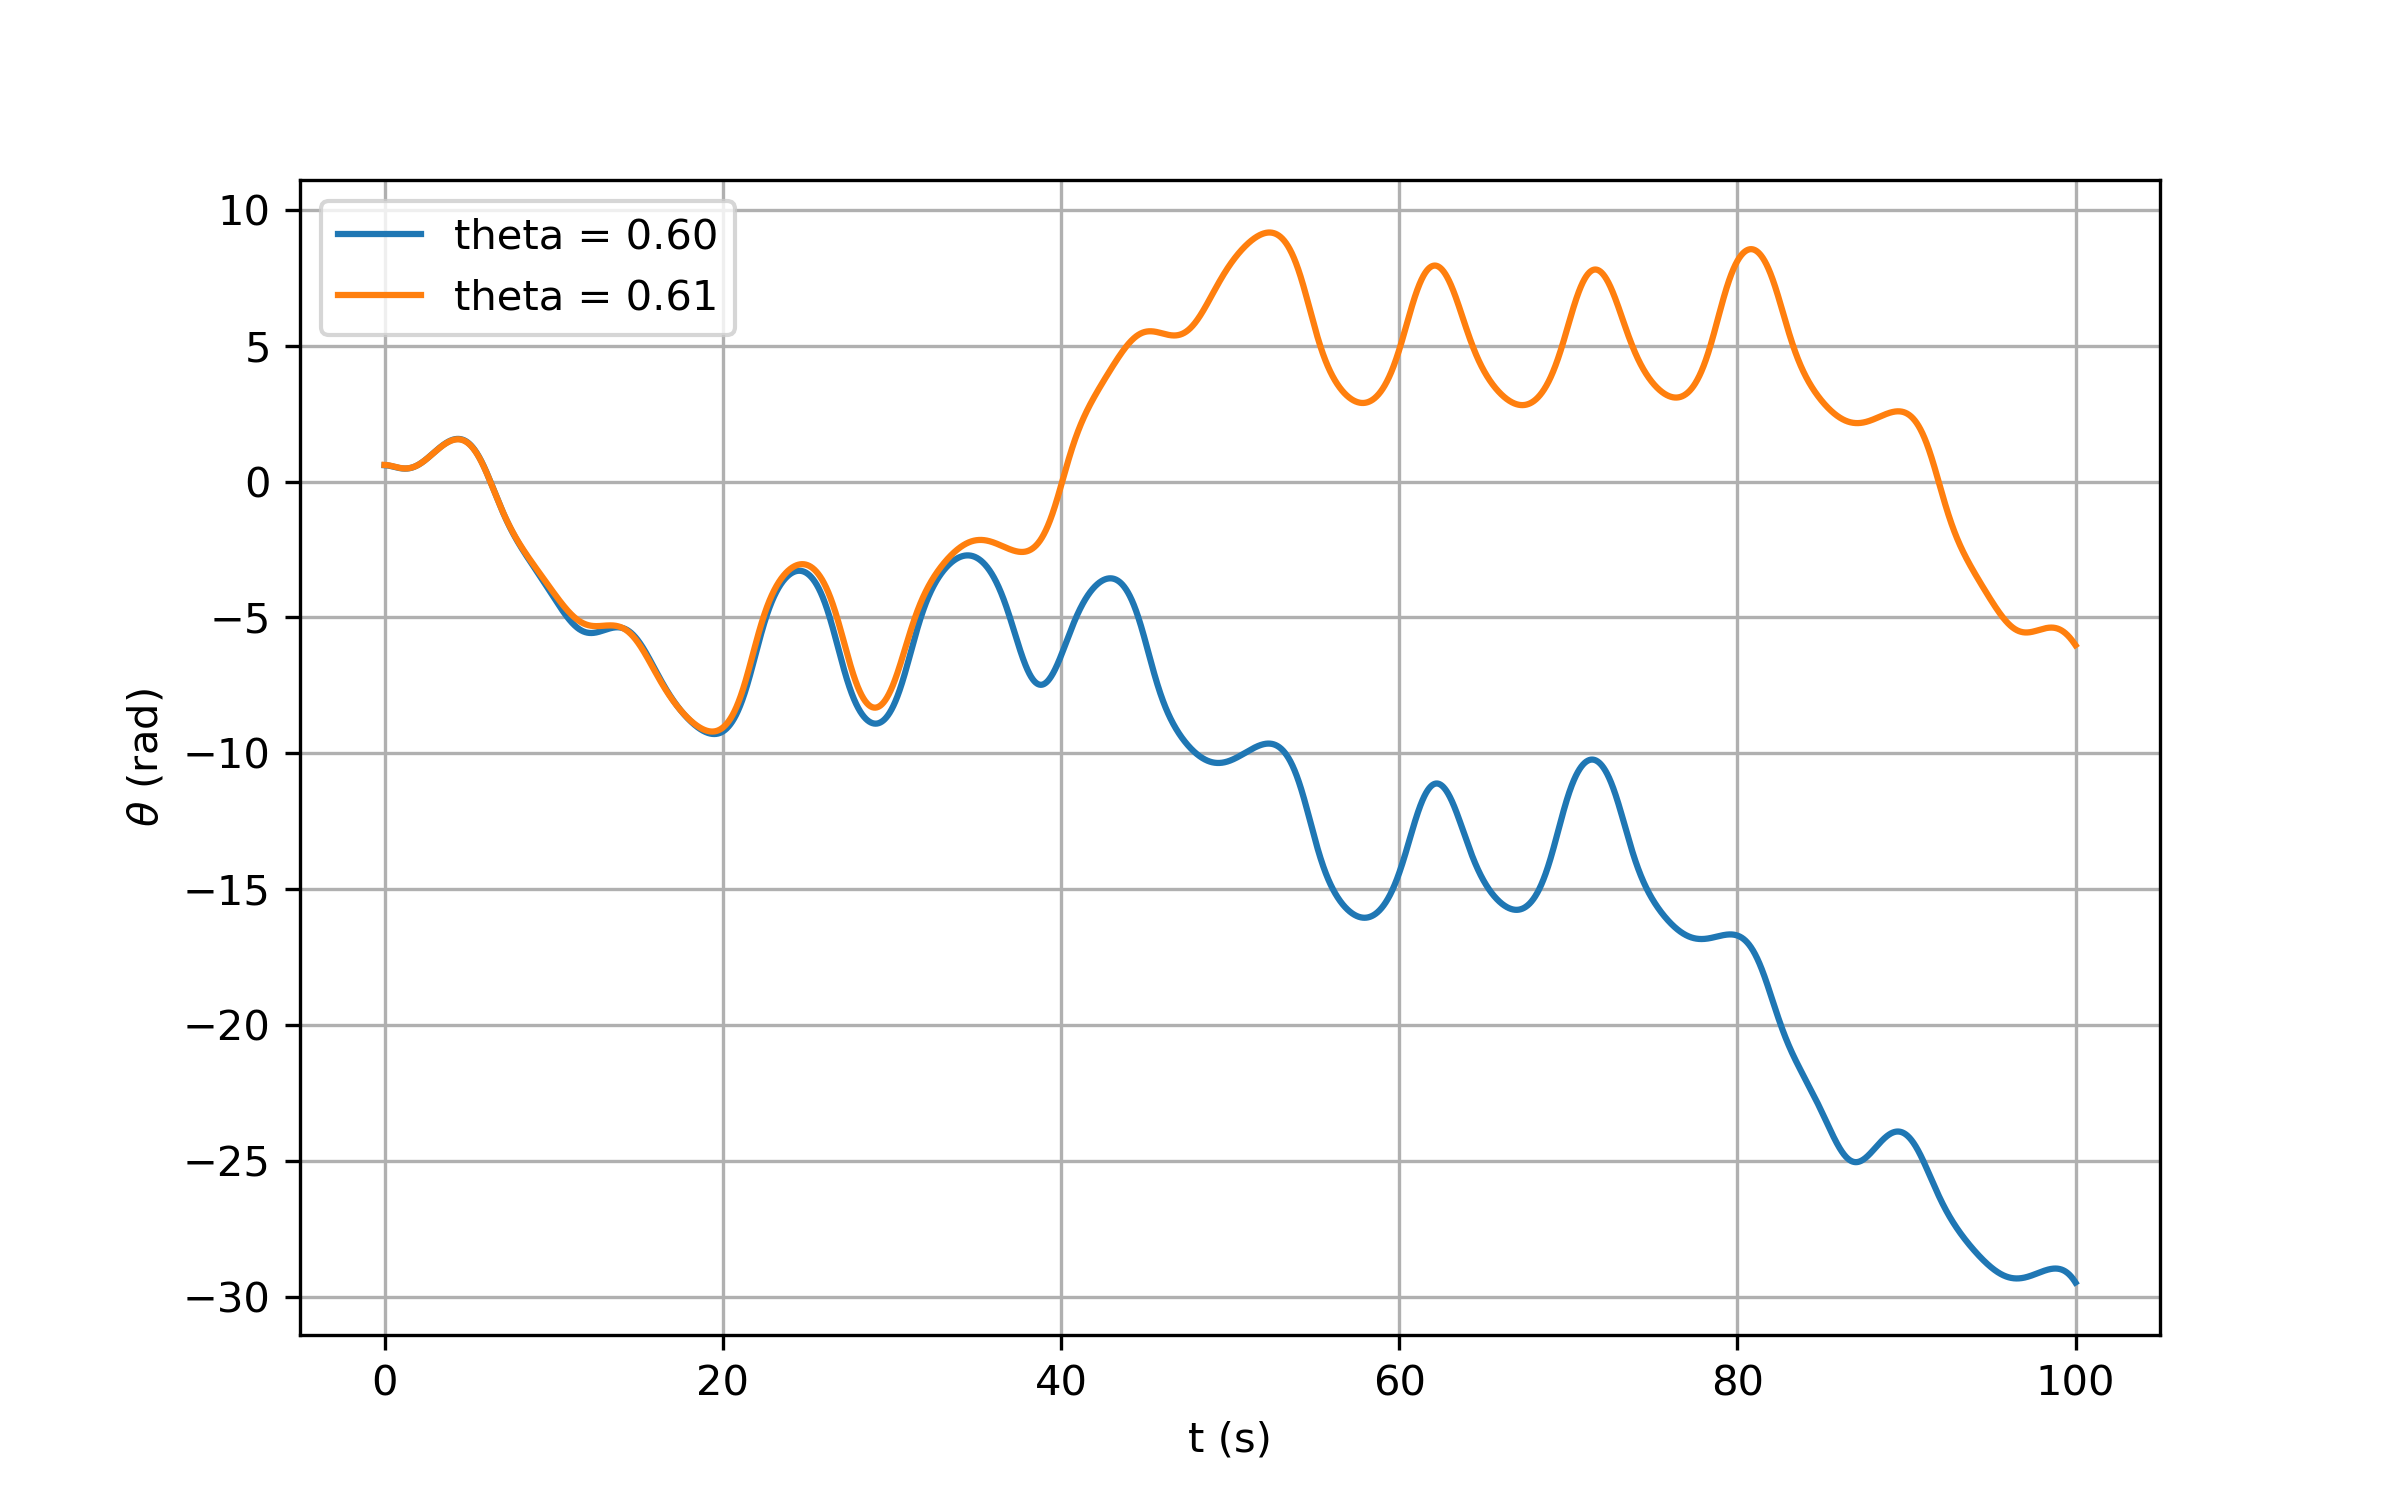
\includegraphics[width=\linewidth]{imagenes_4/comp_ci_b_0.60.png}
    \caption{$\theta = 0.60$}
\end{subfigure}

\caption{Amplitud angular del péndulo en función del tiempo}
\label{fig:comparacion}
\end{figure}

\begin{figure}[H]
\centering
\begin{subfigure}{0.32\textwidth}
    \centering
    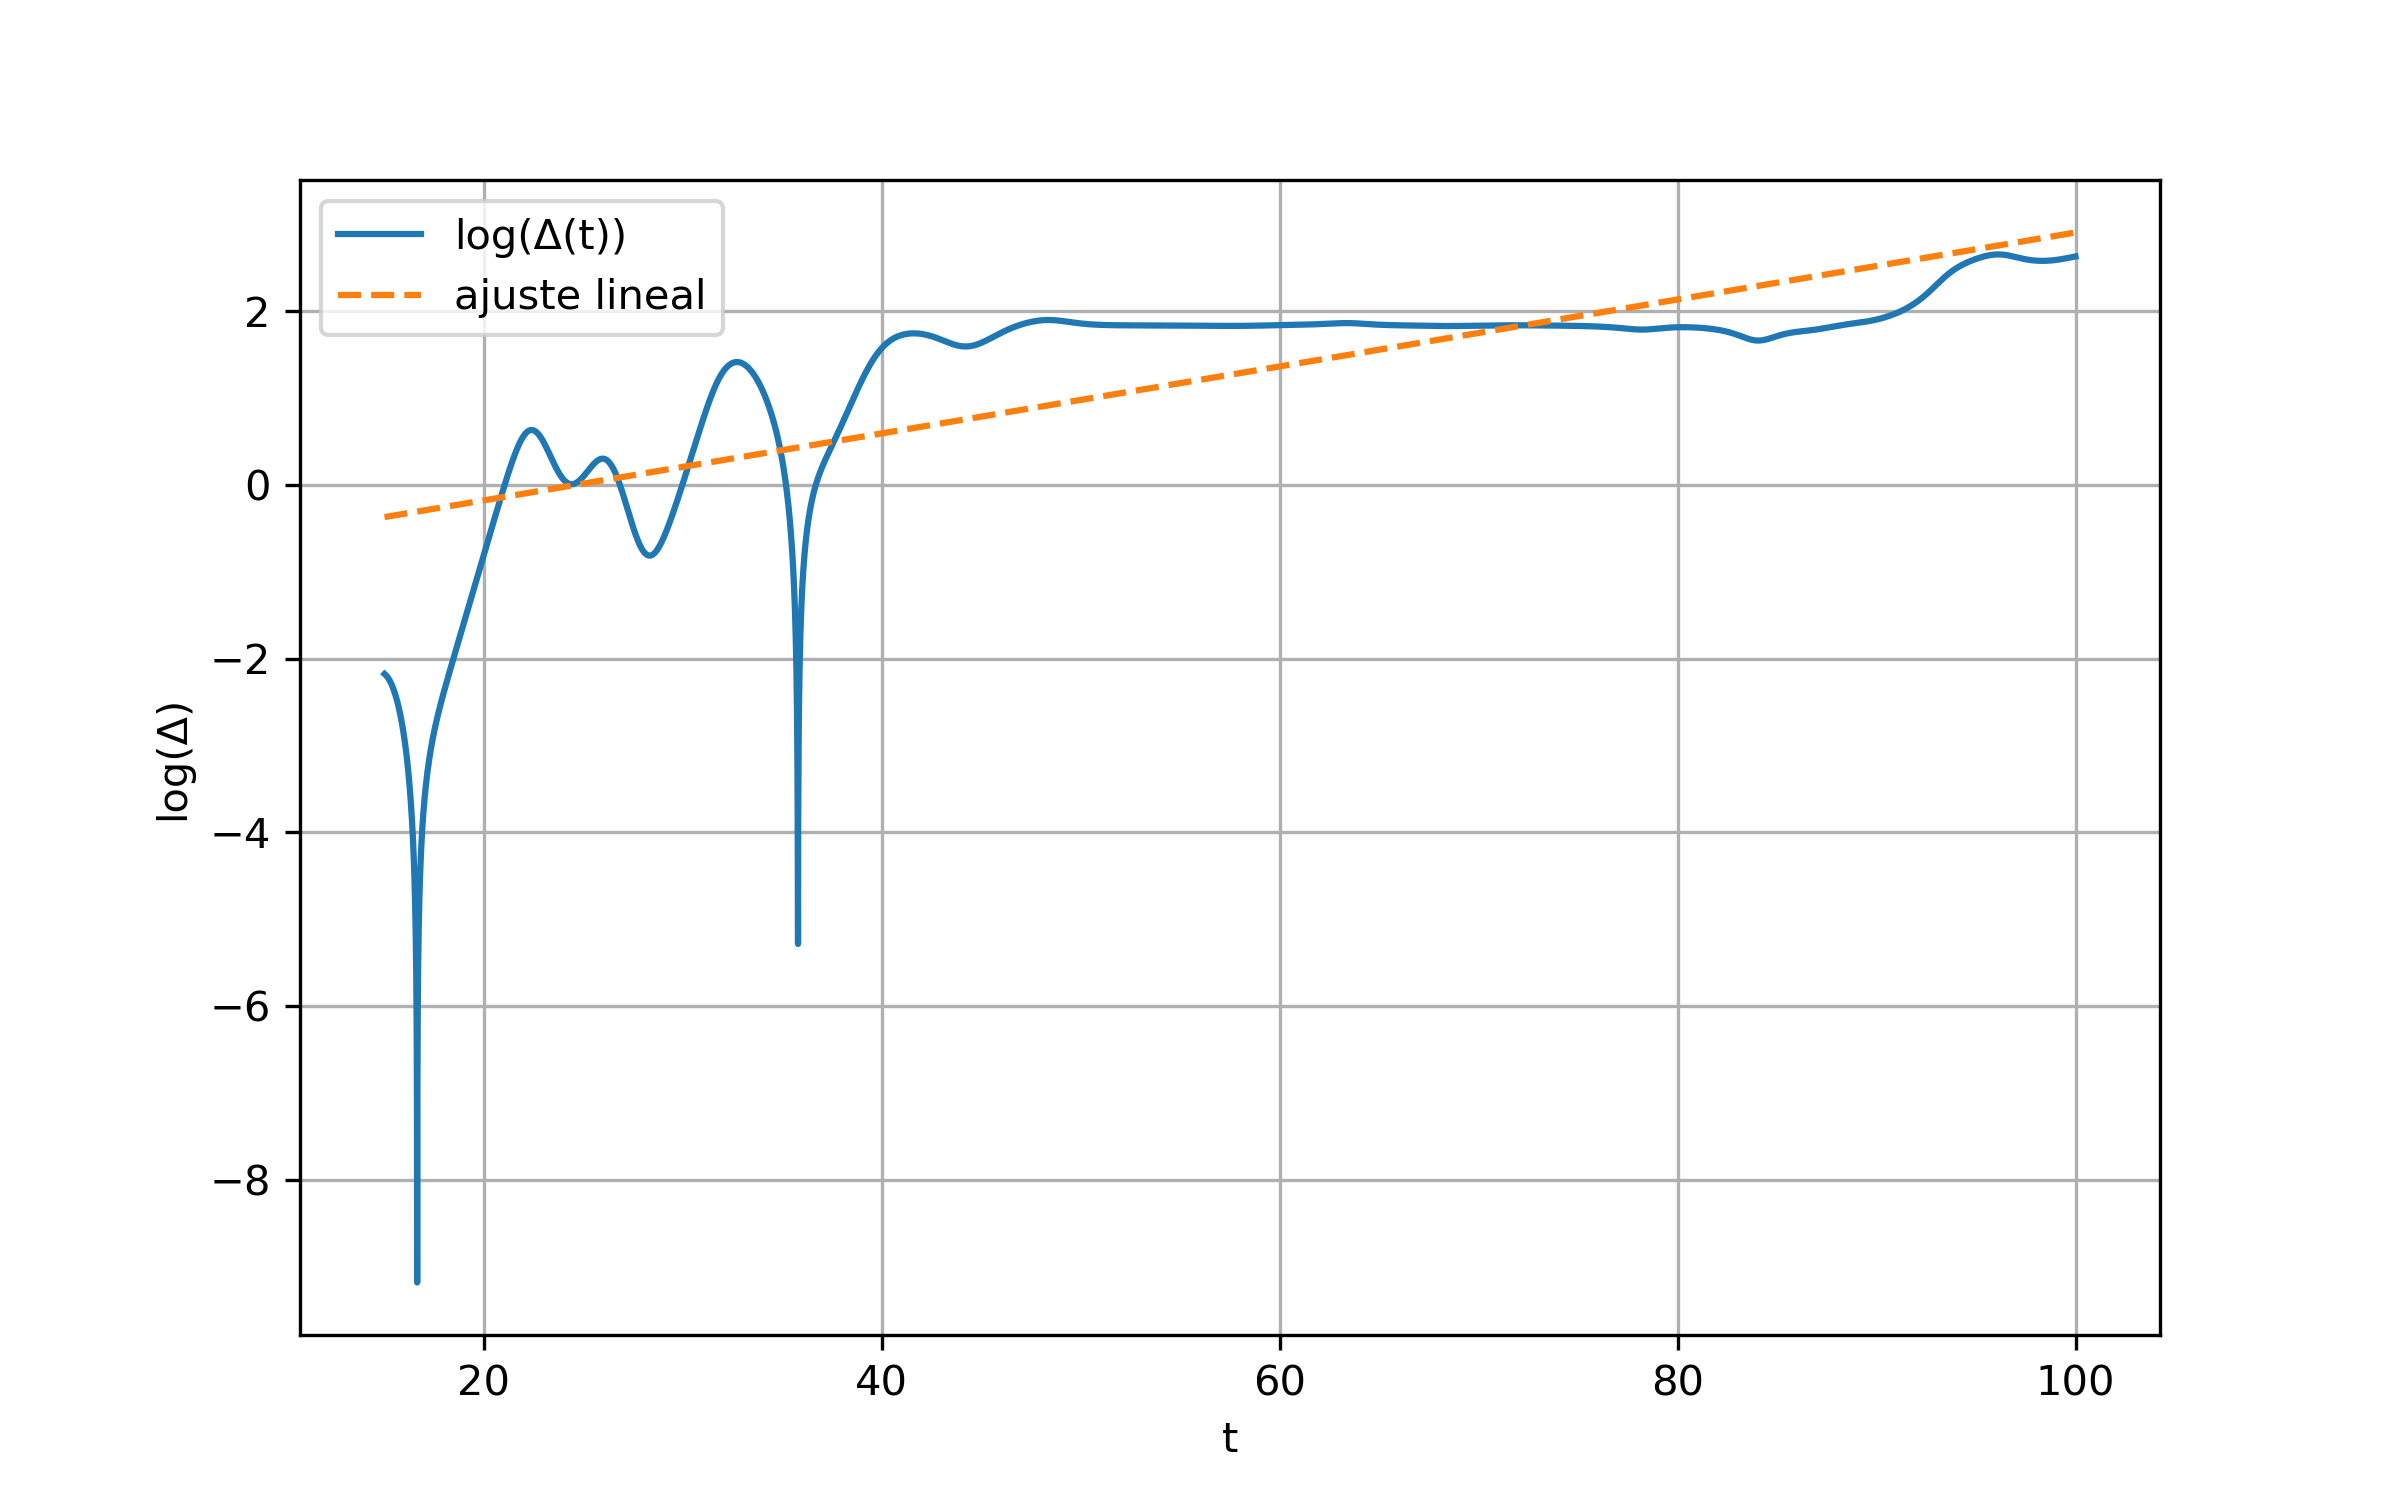
\includegraphics[width=\linewidth]{imagenes_4/apartado_b_theta_0.20.png}
    \caption{$\theta = 0.20$}
\end{subfigure}
\hfill
\begin{subfigure}{0.32\textwidth}
    \centering
    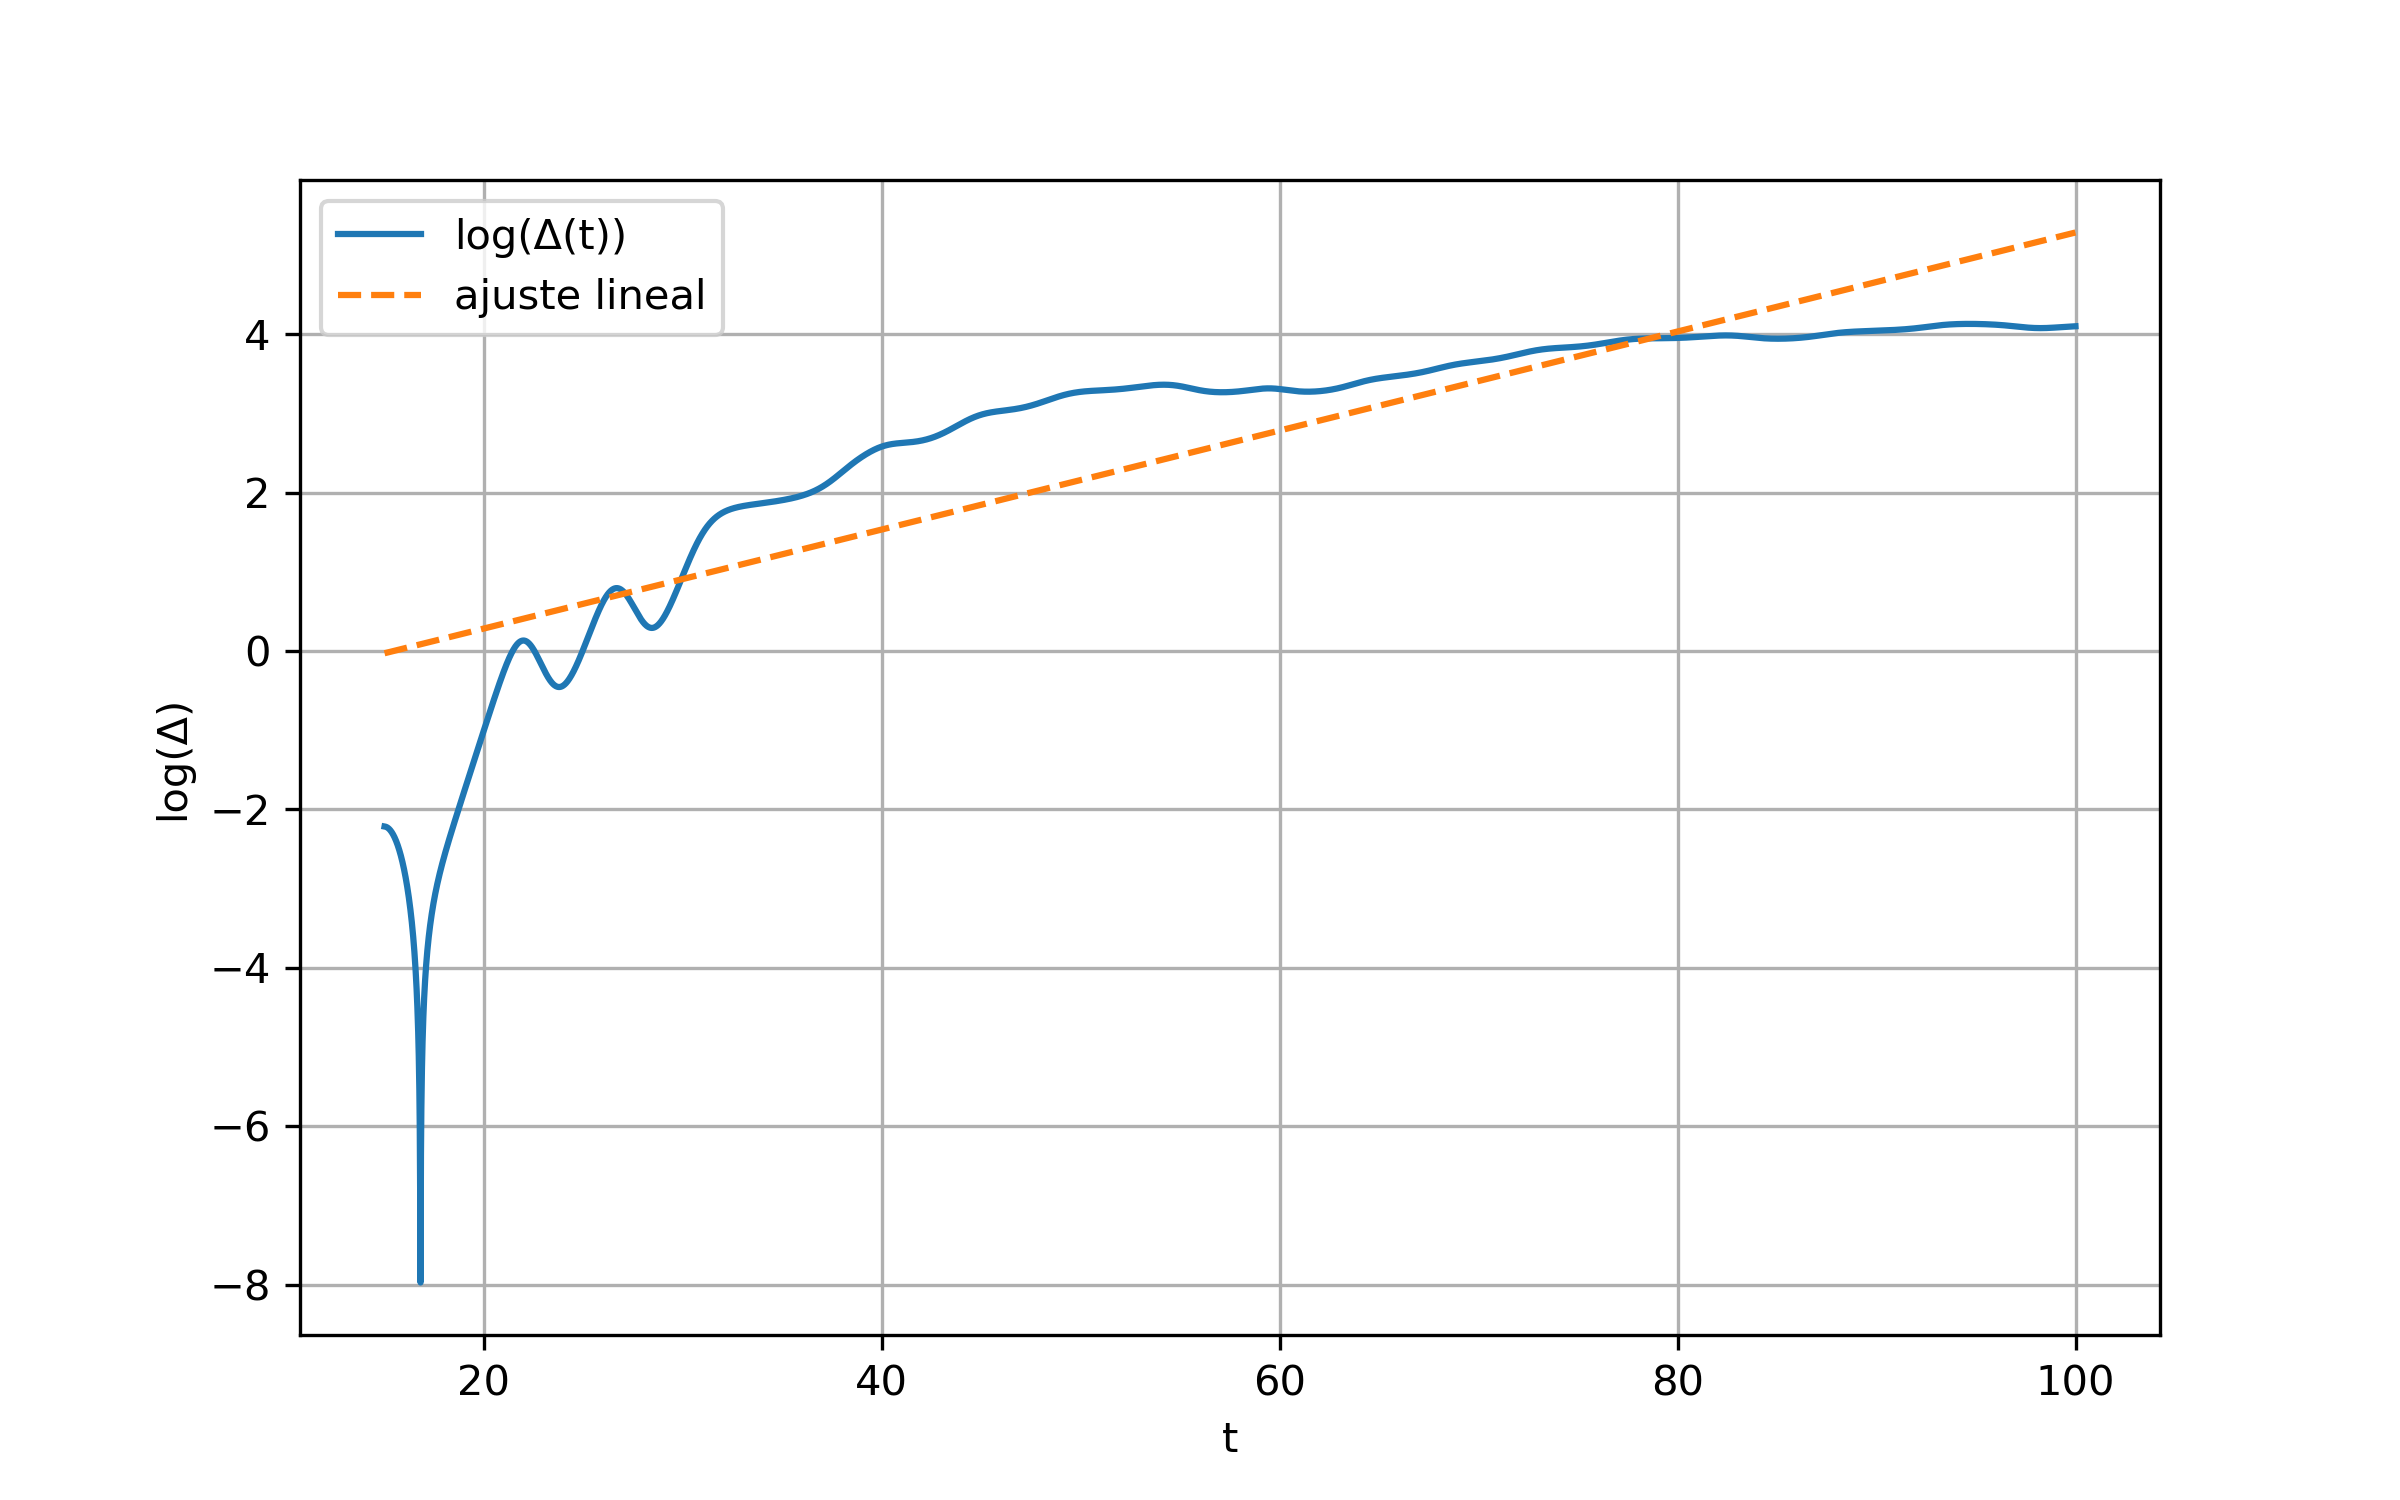
\includegraphics[width=\linewidth]{imagenes_4/apartado_b_theta_0.40.png}
    \caption{$\theta = 0.40$}
\end{subfigure}
\hfill
\begin{subfigure}{0.32\textwidth}
    \centering
    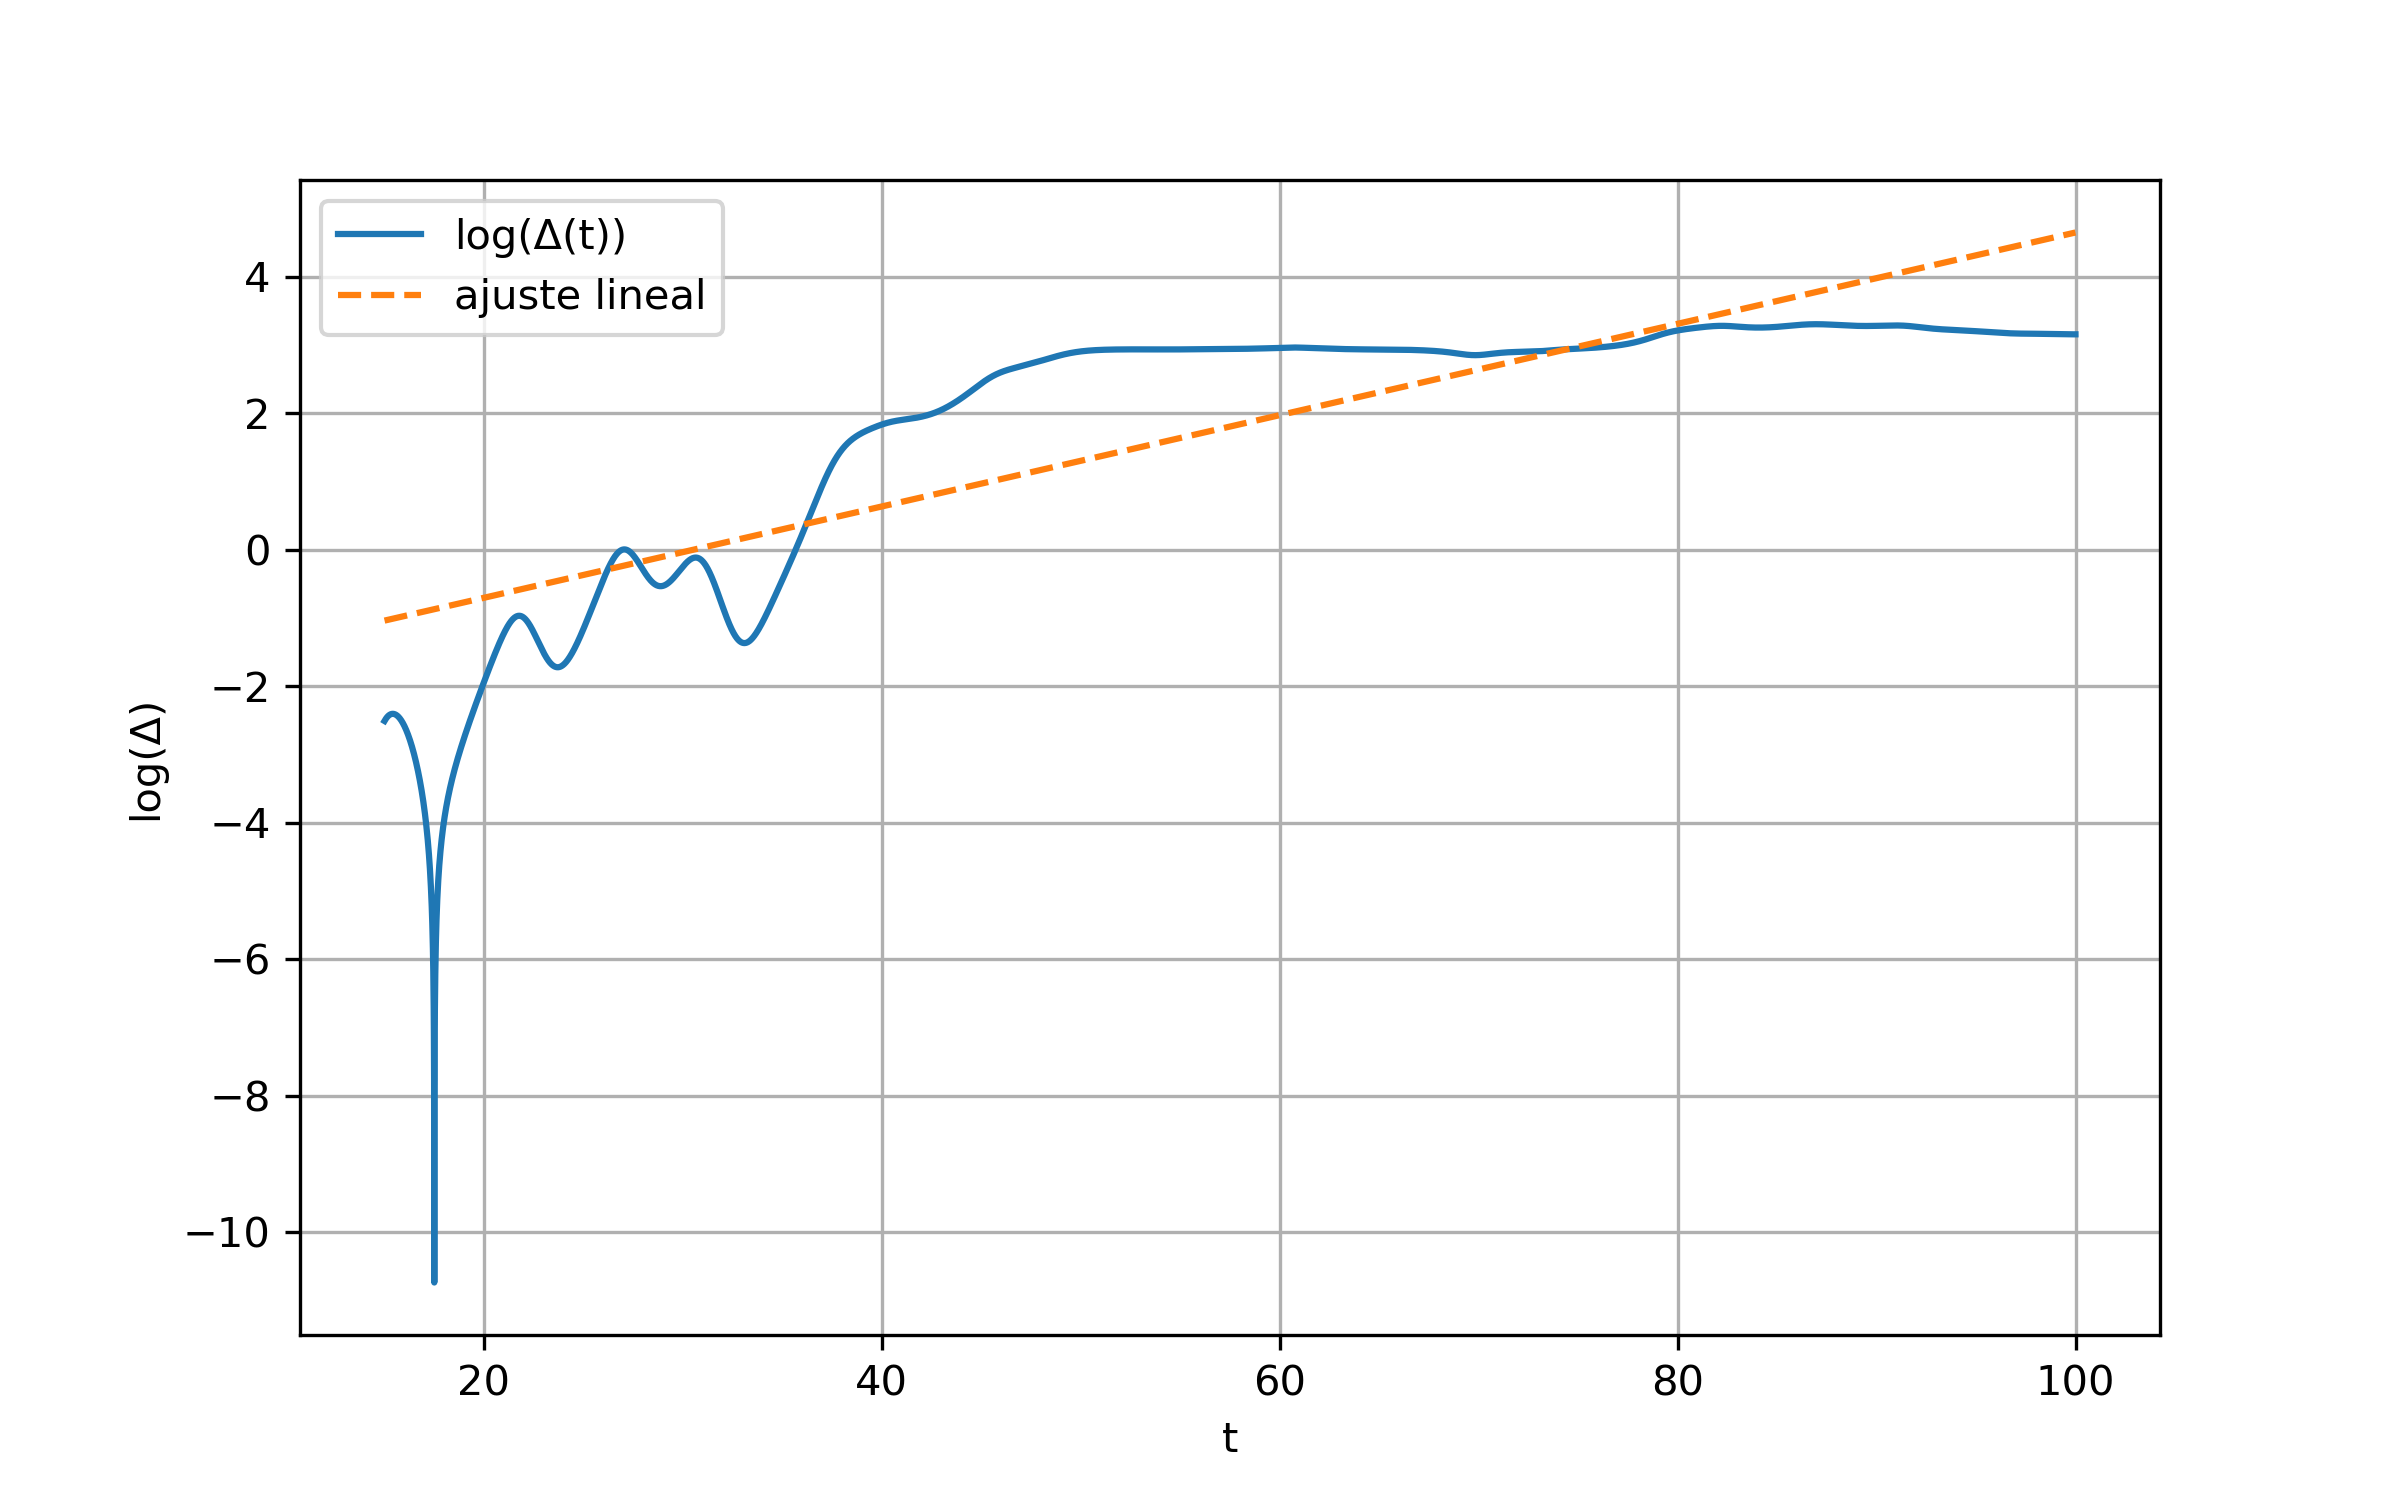
\includegraphics[width=\linewidth]{imagenes_4/apartado_b_theta_0.60.png}
    \caption{$\theta = 0.60$}
\end{subfigure}

\caption{Obtención de los exponentes de Lyapunov}
\label{fig:comparacion}
\end{figure}

El valor estimado del exponente de Lyapunov obtenido es:

\[
\lambda = 0.071 \pm 0.019>0
\]

Se observa que la divergencia entre trayectorias sigue siendo exponencial, aunque su en el estado transitorio parece menor y alcanza un régimen caótico en menos tiempo (respaldado por un exponente de Lyapunov mayor que 0 en los tres casos).

Esto indica que pequeñas variaciones en el amortiguamiento afectan a la dinámica del sistema, pero, al menos en este caso, el sistema permanece en régimen caótico.

Para estudiar la variación de la dinámica del sistema en función del amortiguamiento se puede representar el coeficiente de Lyapunov en función del coeficiente de amortiguamiento:

\begin{figure}[H]
\centering
\begin{subfigure}{0.32\textwidth}
    \centering
    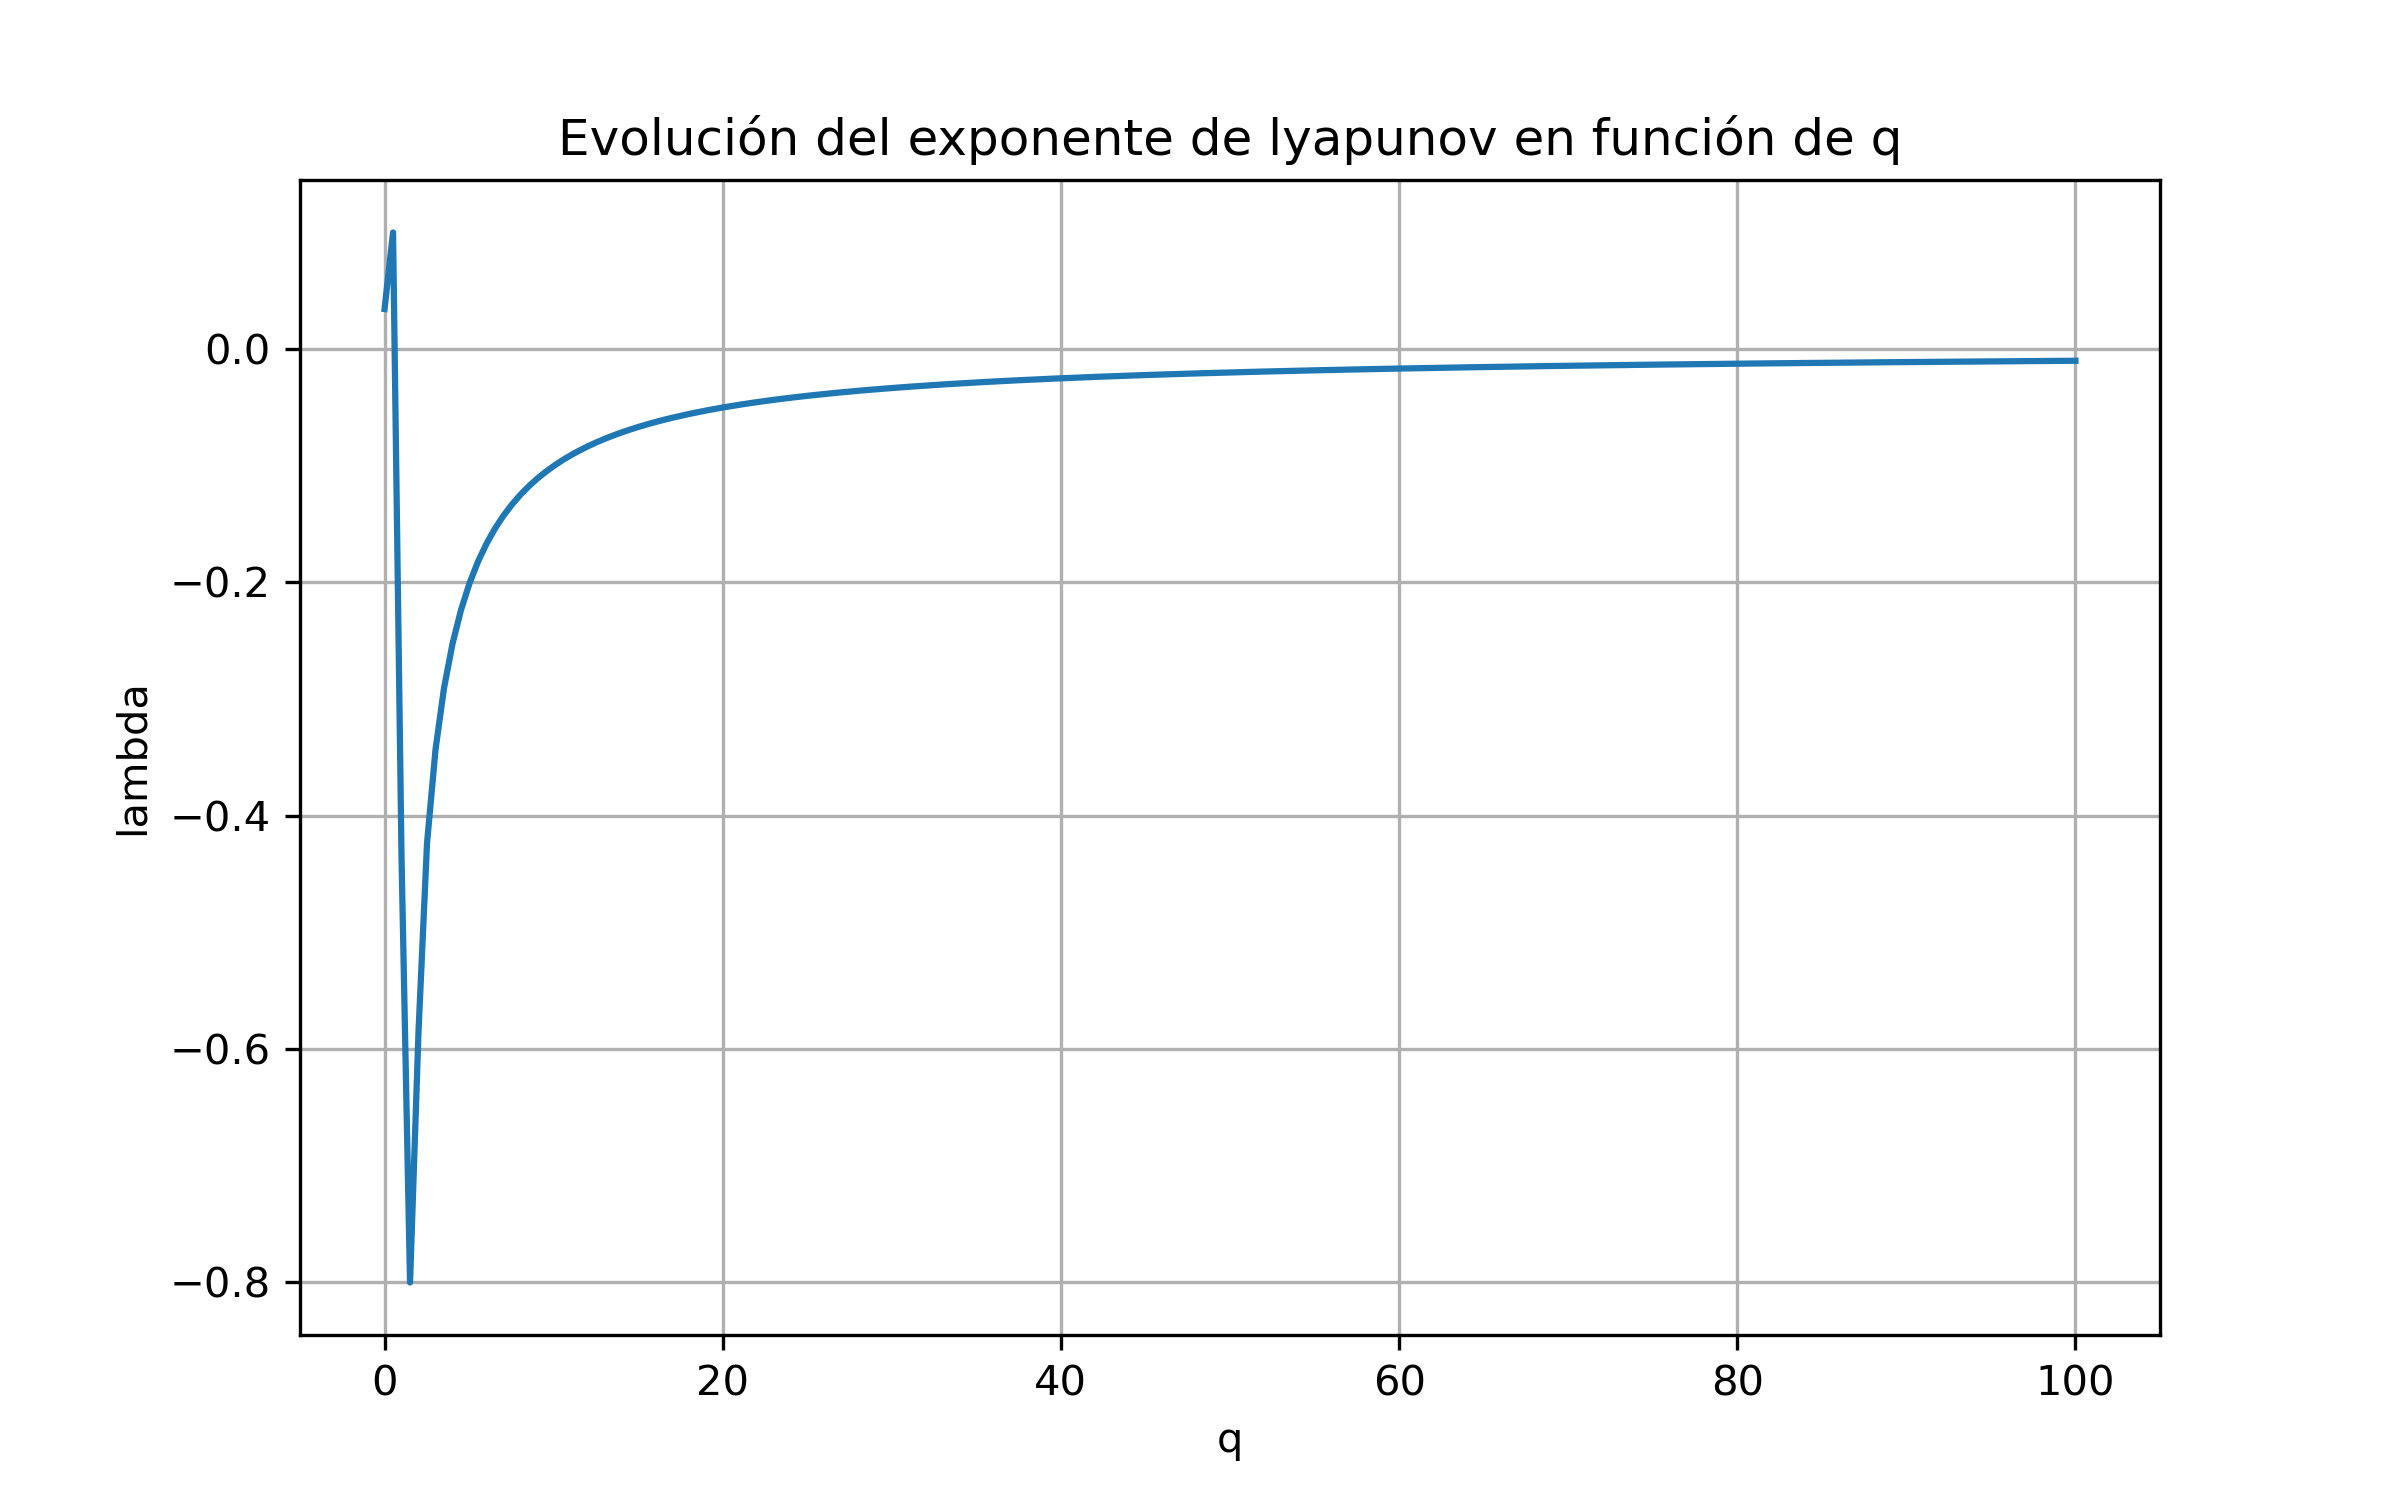
\includegraphics[width=\linewidth]{imagenes_4/lyapunov(q).png}
    \caption{Vista general}
    \label{fig:general}
\end{subfigure}
\hfill
\begin{subfigure}{0.32\textwidth}
    \centering
    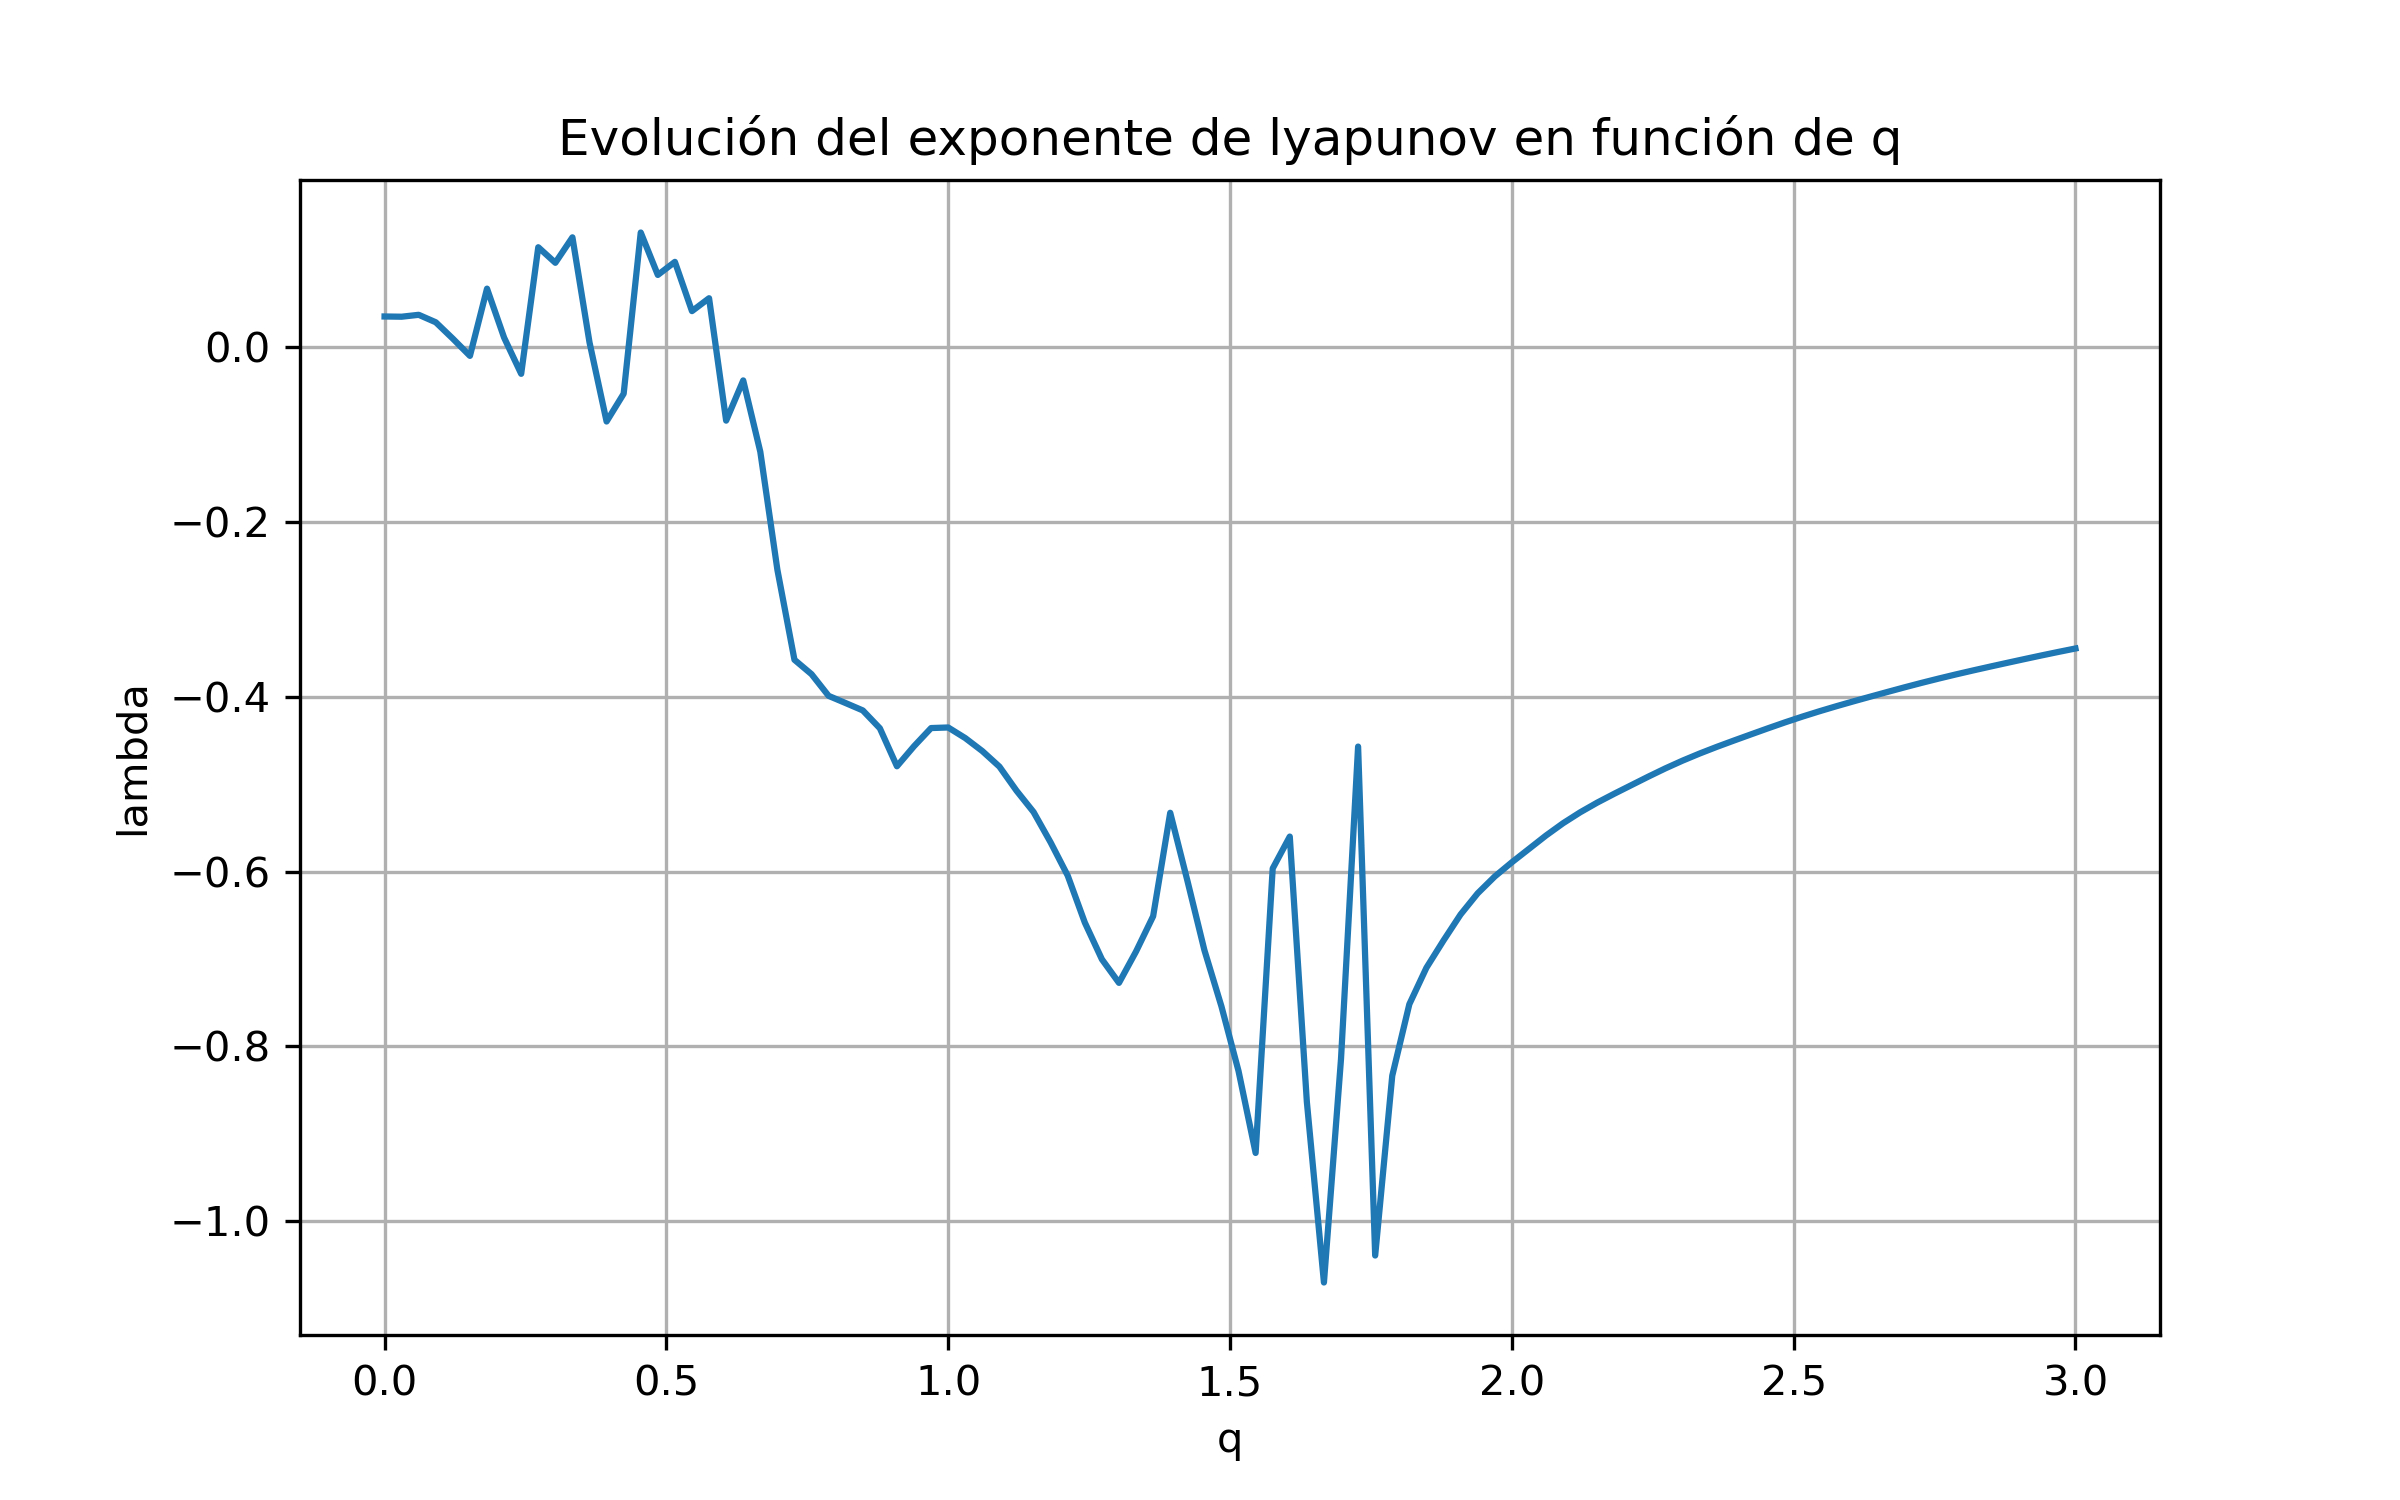
\includegraphics[width=\linewidth]{imagenes_4/zoom_general_lyapunov(q).png}
    \caption{$q\leq 3$}
    \label{fig:zoomgeneral}
\end{subfigure}
\hfill
\begin{subfigure}{0.32\textwidth}
    \centering
    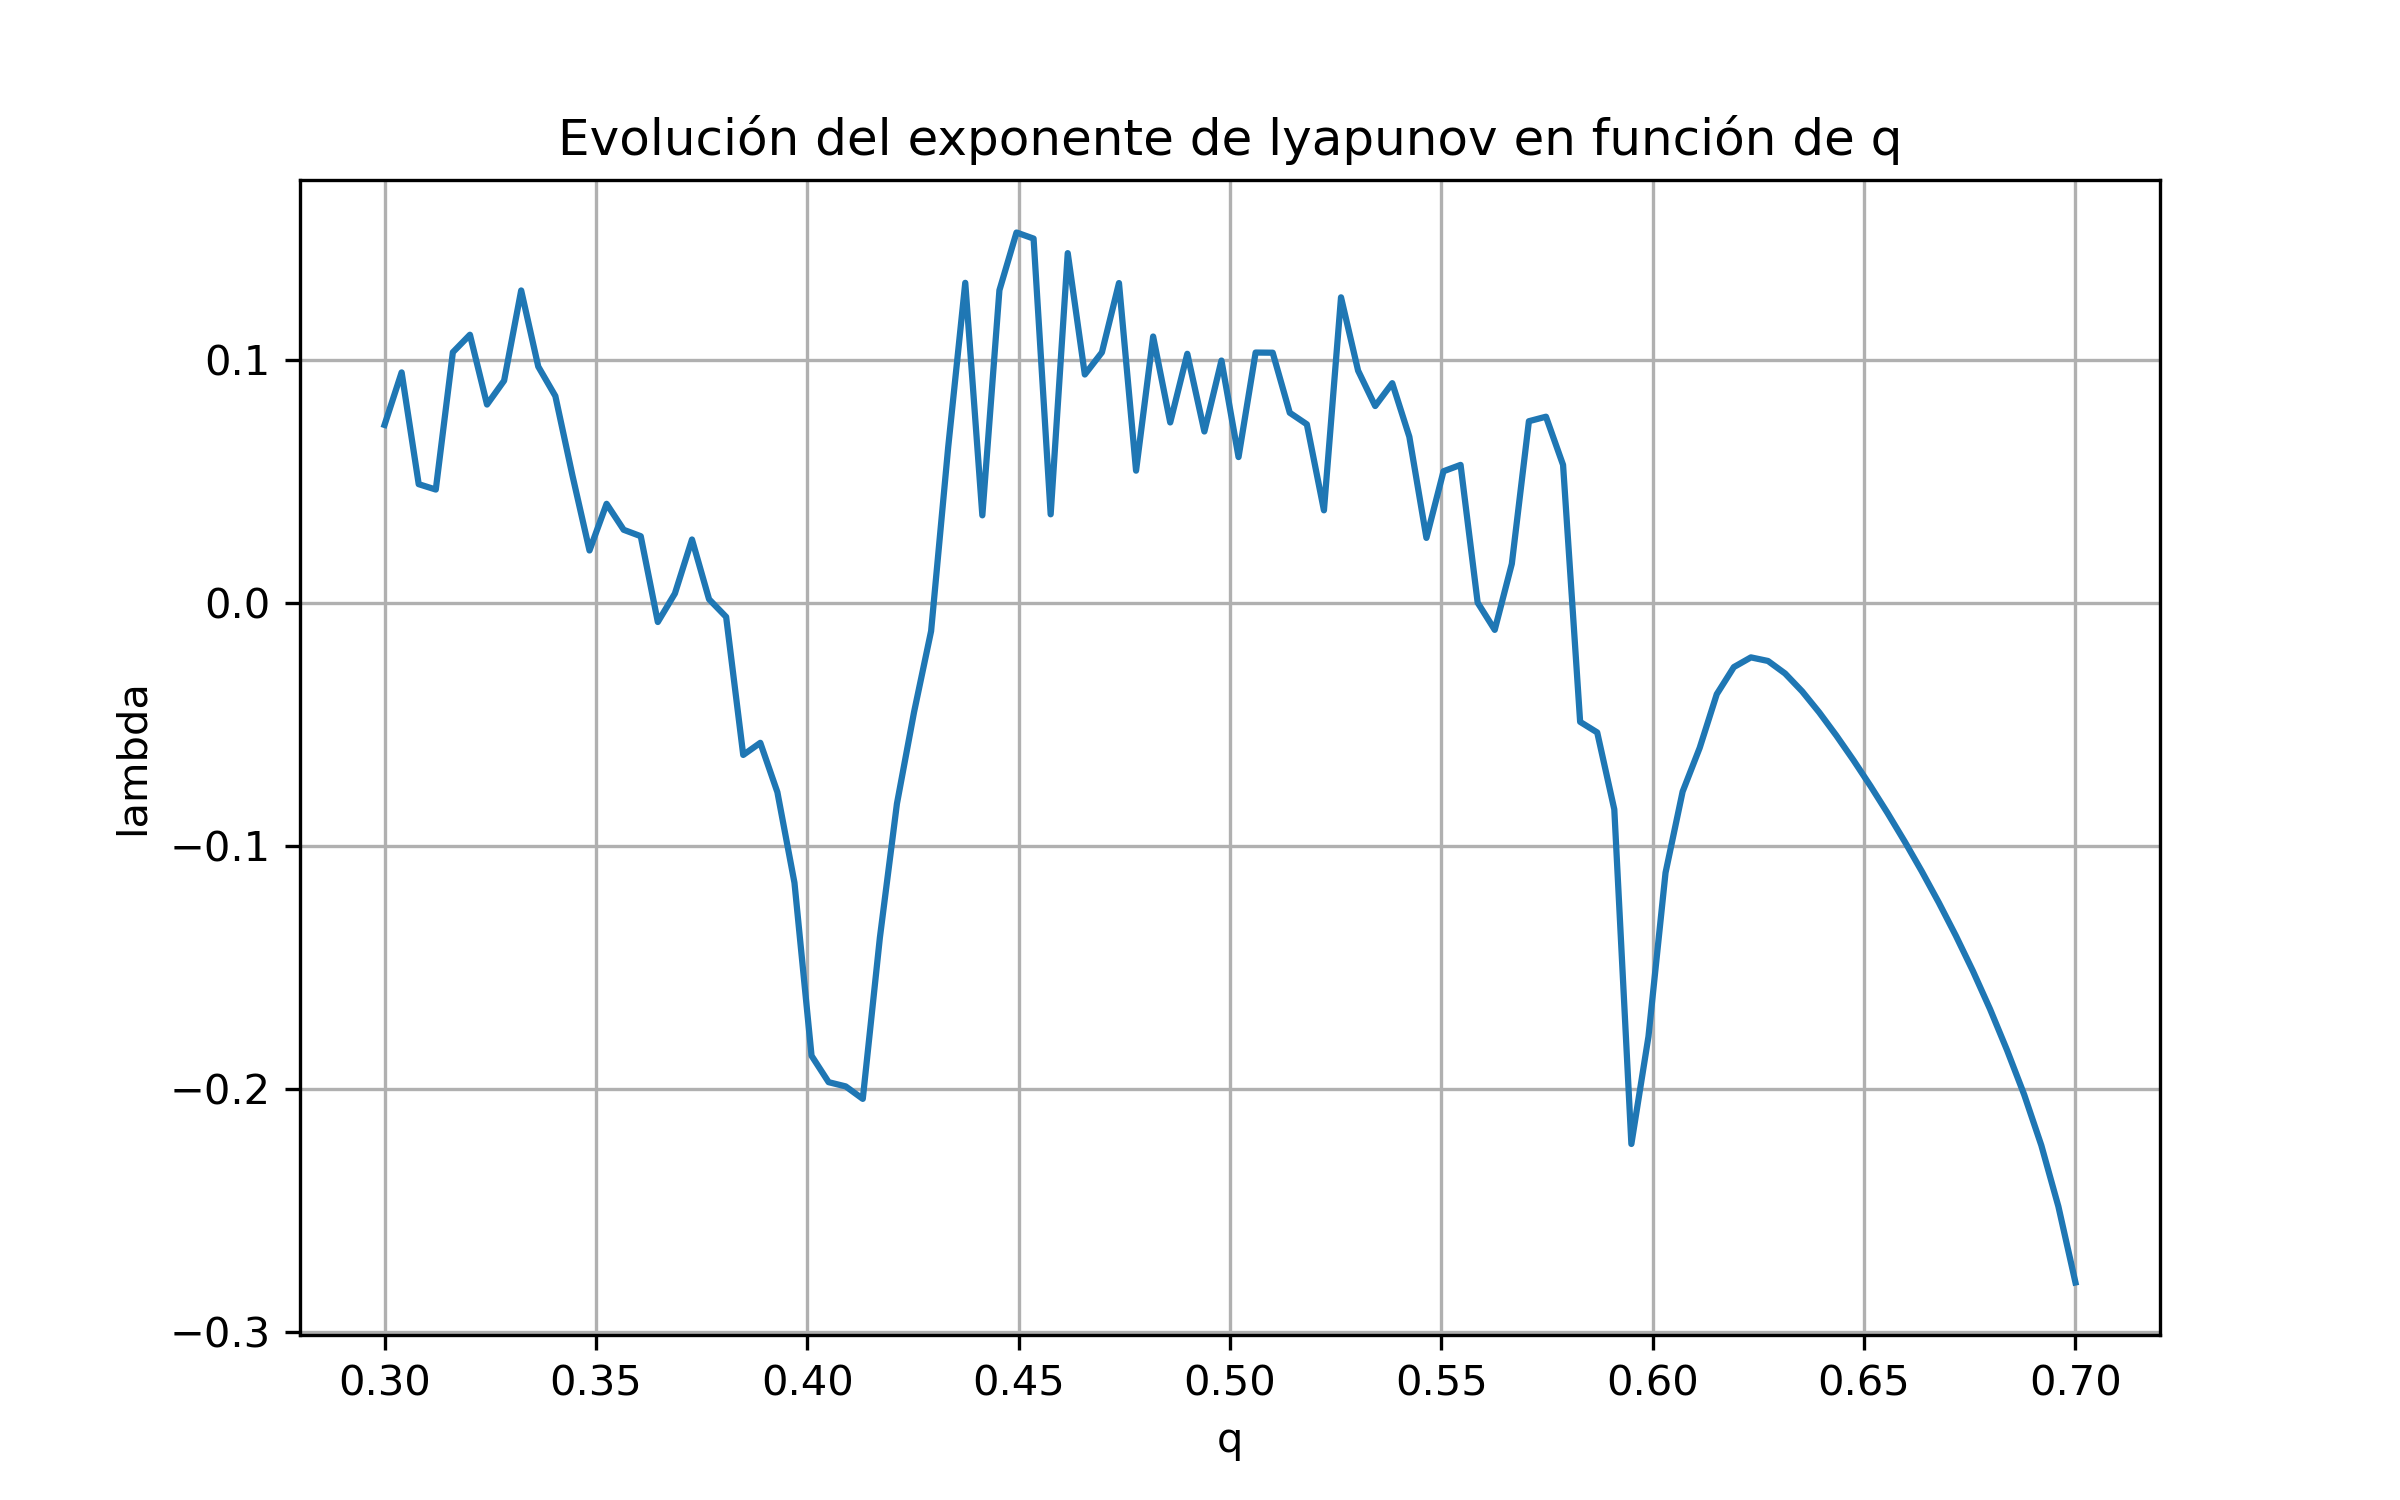
\includegraphics[width=\linewidth]{imagenes_4/zoom_qsub_lyapunov(q).png}
    \caption{$0.3 \leq q \leq 0.6$}
    \label{fig:zoomespecifico}
\end{subfigure}

\caption{Evolución del exponente de Lyapunov en función de q}
\label{fig:comparacion}
\end{figure}

En estos gráficos se observa que el aumento del amortiguamiento puede hacer que el sistema, inicialmente en régimen caótico pase a un régimen oscilatorio. Además, como se ve en \ref{fig:general}, cuando el amortiguamiento es suficientemente grande, el coeficiente de Lyapunov es prácticamente 0 debido a que el sistema está completamente sobreamortiguado y las amplitudes de ambos péndulos tienden a 0 rápidamente. Si nos centramos en \ref{fig:comparacion}, observamos que para $q>0.58$, el sistema se encuentra en régimen oscilatorio. Finalmente, observando \ref{fig:zoomespecifico}, se ratifica que en el apartado b) de la práctica el sistema se encuentra en régimen caótico.

\subsection{Diagrama de bifurcación}

Finalmente, para estudiar también la transición hacia el caos mediante la variación de la fuerza impulsora, se construyó un diagrama de bifurcación en el intervalo:

\[
1.1 \le F_I \le 1.6
\]

Los puntos del diagrama corresponden a valores del ángulo registrados cada periodo de la fuerza impulsora tras eliminar el régimen transitorio.

\begin{figure}[H]
\centering
\begin{subfigure}{0.49\textwidth}
    \centering
    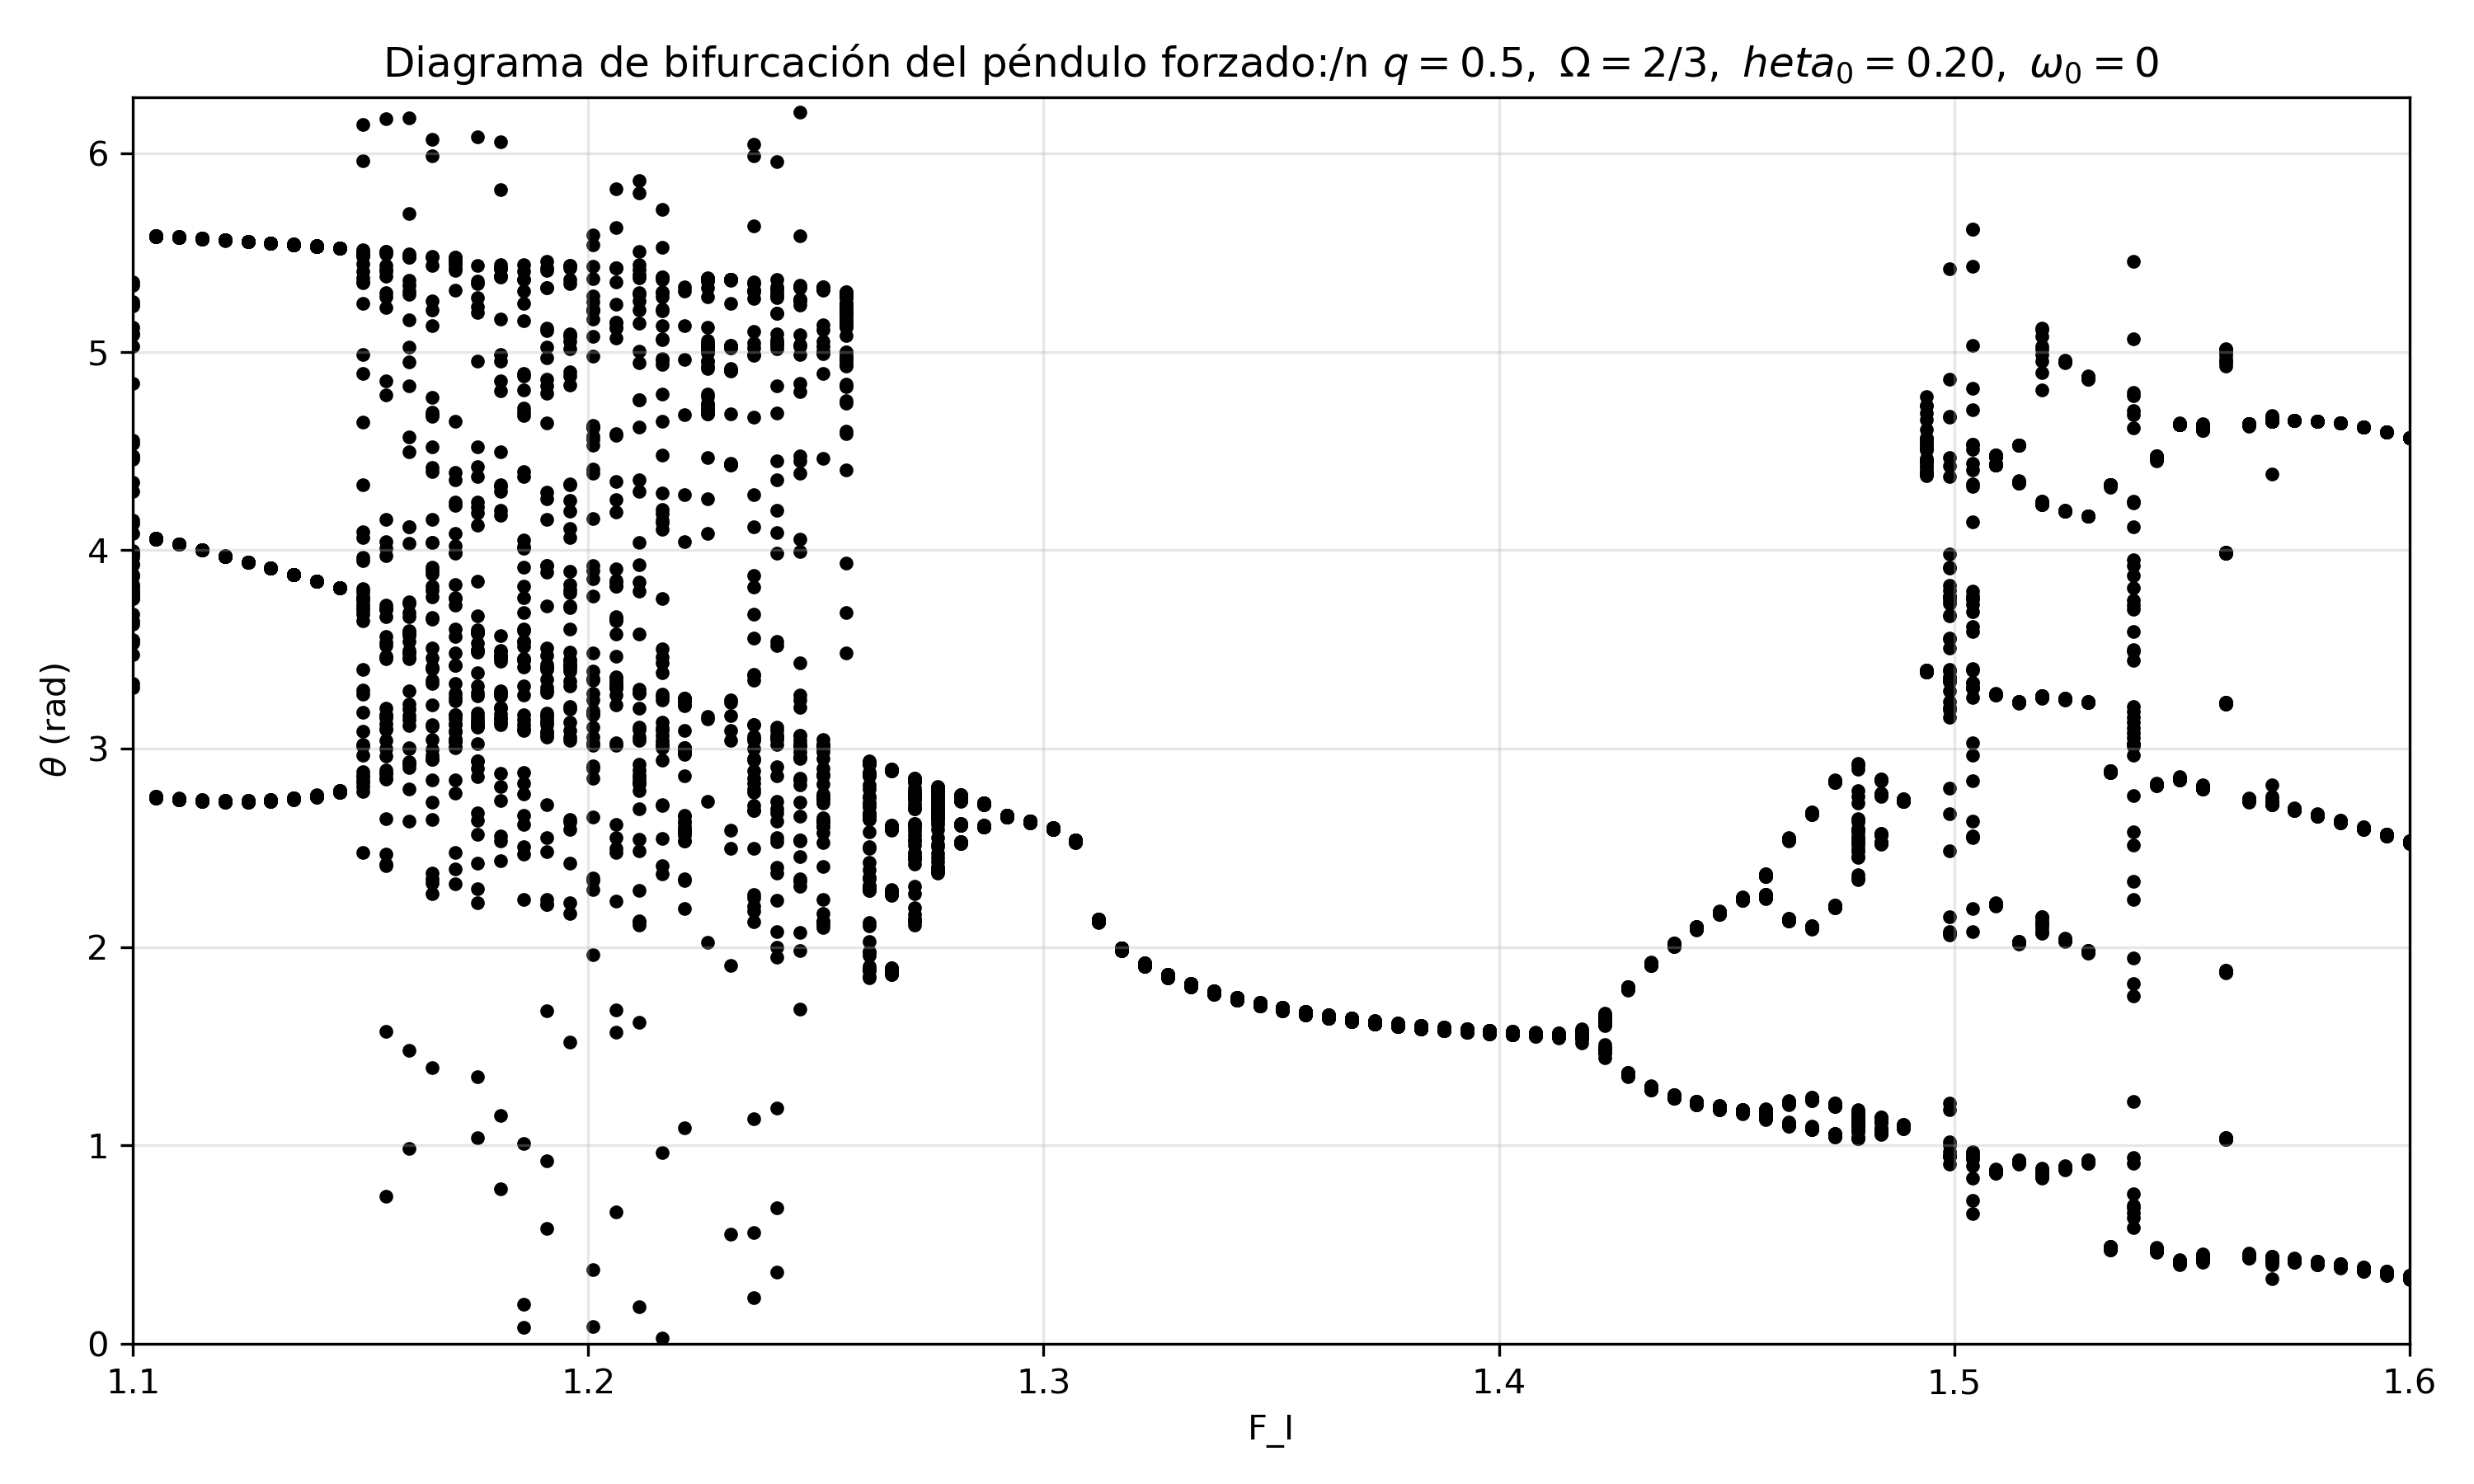
\includegraphics[width=0.9\textwidth]{imagenes_4/bif.png}
    \caption{$1.1 \le F_I \le 1.6$}
    \label{bif_completo}
\end{subfigure}
\hfill
\begin{subfigure}{0.49\textwidth}
    \centering
    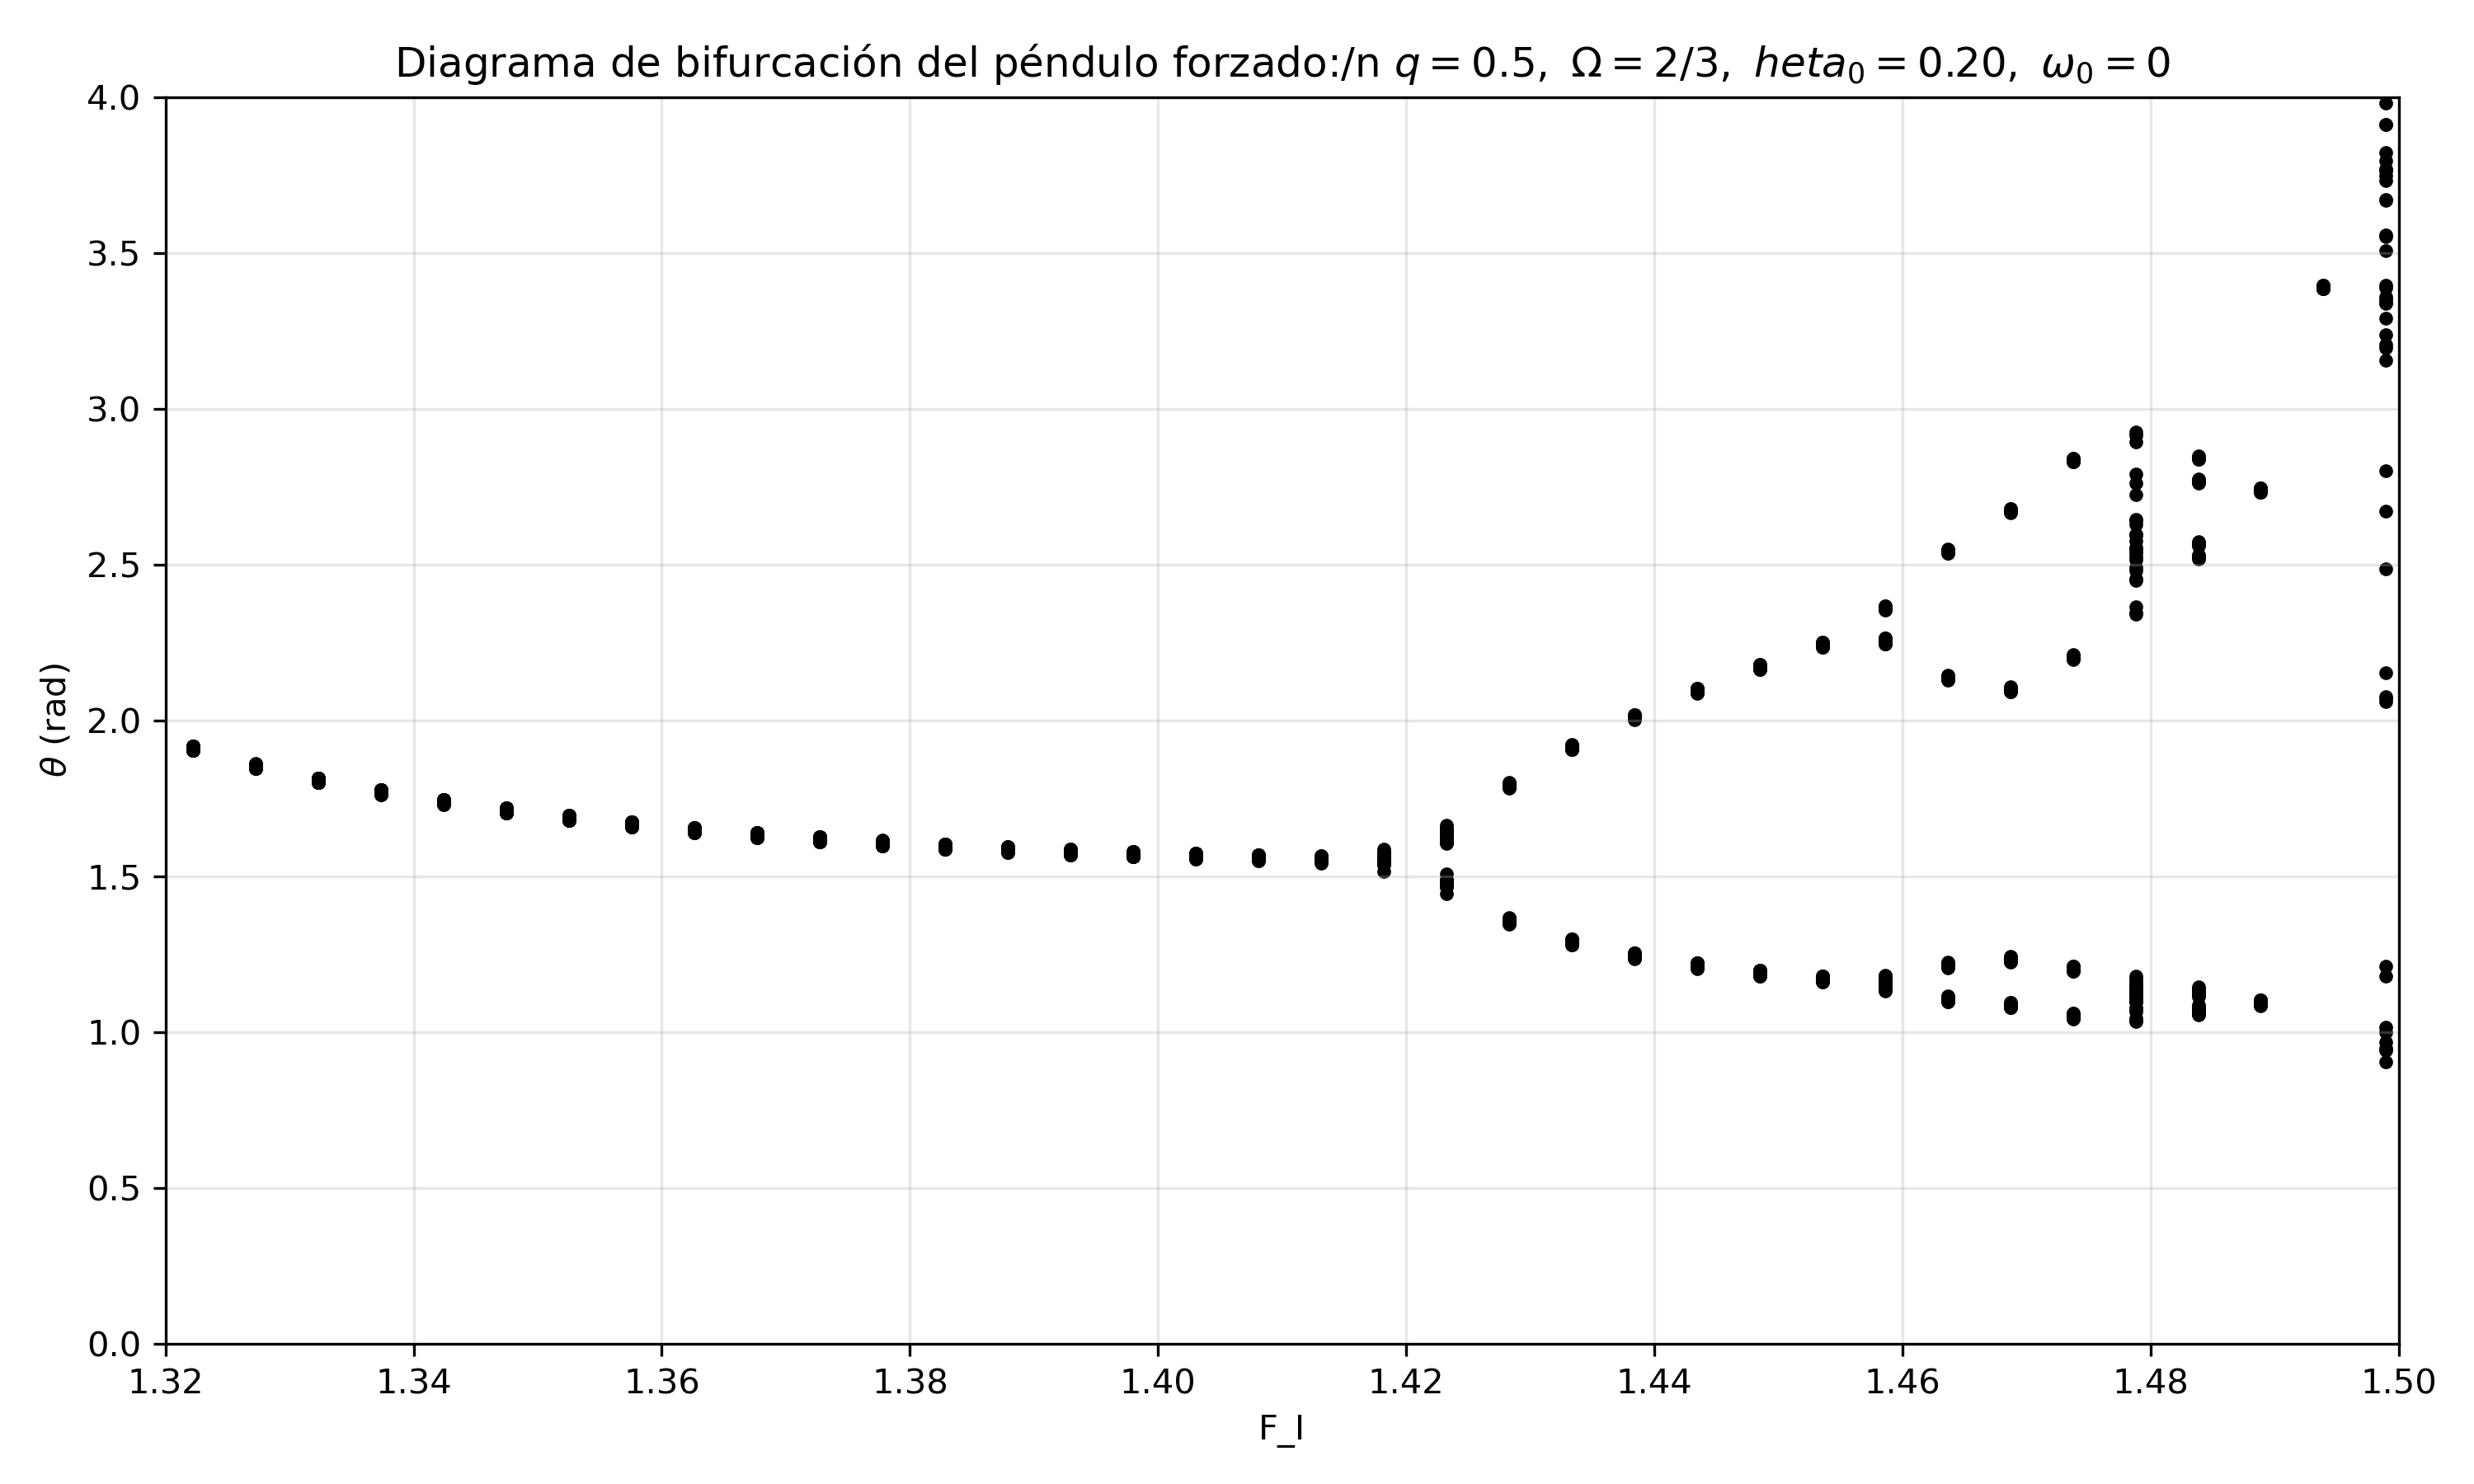
\includegraphics[width=\linewidth]{imagenes_4/bif_zoom.png}
    \caption{$1.32 \leq F_I \leq 1.5$}
    \label{zoombif}
\end{subfigure}
\hfill
\caption{Diagrama de bifurcación de un péndulo no lineal}
\label{fig:comparacion}
\end{figure}



En el diagrama \ref{bif_completo} se verifica nuevamente que cuando $F_I=1.2$, el sistema sugerido se encuentra en régimen caótico.

Además, resulta interesante observar el rango $1.32 \leq F_I \leq 1.5$ ya que se produce la transición al régimen caótico mediante el duplicado del periodo. En ese rango, el sistema sugerido comienza en régimen oscilatorio, duplica su periodo en $F_I\approx 1.42$, vuelve a duplicar su periodo en $F_I\approx 1.46$ y finalmente, entra en régimen caótico en $F_I\approx 1.48$.

\section{Conclusiones}

El estudio numérico del péndulo no lineal sugerido nos lleva al estudio de un sistema caótico. Además, se ha comprobado la bondad del exponente de Lyapunov y el diagrama de bifurcación para predecir el régimen de un sistema dinámico dado tras atravesar el régimen transitorio inicial.

Además, se ha estudiado la evolución del exponente de Lyapunov con el aumento del amortiguamiento, concluyendo que el aumento del amortiguamiento puede evitar que un sistema entre en régimen caótico.

Finalmente, se ha observado un diagrama de bifurcación del modelo sugerido y cómo a través de duplicar su periodo un sistema dinámico puede pasar de régimen oscilatorio a régimen caótico.


\begin{thebibliography}{9}

\bibitem{giordano}
N. J. Giordano and H. Nakanishi,
\textit{Computational Physics},
2nd ed., Pearson Prentice Hall, 2006.
\label{giordano}
\end{thebibliography}

\newpage
\appendix
\section*{Anexo A: Variables y condiciones iniciales empleadas}

\addcontentsline{toc}{section}{Anexo A: Variables y condiciones iniciales empleadas}

\begin{table}[H]
\centering
\begin{tabular}{ll}
\toprule
Símbolo & Significado físico \\
\midrule
$\theta$ & Ángulo del péndulo \\
$\omega$ & Velocidad angular \\
$q$ & Coeficiente de amortiguamiento \\
$F_I$ & Amplitud de la fuerza impulsora \\
$\Omega_I$ & Frecuencia angular de la fuerza externa \\
$l$ & Longitud del péndulo \\
$g$ & Aceleración gravitatoria \\
$\Delta t$ & Paso temporal de integración \\
$\lambda$ & Exponente de Lyapunov \\
\bottomrule
\end{tabular}
\caption{Variables empleadas en el desarrollo teórico y numérico.}
\end{table}

\begin{table}[H]
\centering
\begin{tabular}{ll}
\toprule
Parámetro & Valor utilizado \\
\midrule
$l$ & $9.8m$ \\
$g$ & $9.8 m/s^2$ \\
$\theta_0$ & $0.20$ rad \\
$\omega_0$ & $0$ \\
$q$ & $0.5$ \\
$F_I$ & $1.2N$ \\
$\Omega_I$ & $2/3$ \\
$\Delta t$ & $0.01$ s \\
\bottomrule
\end{tabular}
\caption{Condiciones iniciales utilizadas en las simulaciones.}
\label{tab:ci}
\end{table}

\end{document}